\documentclass[11pt]{article}

\usepackage[utf8]{inputenc}
\usepackage[T1]{fontenc}
\usepackage[a4paper,margin=0.85in]{geometry}
\usepackage{graphicx}
\usepackage{subcaption}
\usepackage{float}
\usepackage{booktabs}
\usepackage{array}
\usepackage{enumitem}
\usepackage{microtype}
\usepackage[hidelinks]{hyperref}
\usepackage{xcolor}
\usepackage{listings}

\usepackage{tikz}
\usetikzlibrary{arrows.meta, positioning, calc, shapes.geometric}

\setlist{nosep,leftmargin=*}
\setlength{\parindent}{0pt}
\setlength{\parskip}{4pt}
\setcounter{tocdepth}{2}

% ---------- Evidence placeholders ----------
% Replace the framed box in any placeholder with, for example:
% \includegraphics[width=\linewidth]{images/phase3_fake_run1.png}
\newcommand{\evidencebox}[1]{%
  \fbox{\parbox[c][4.0cm][c]{0.92\linewidth}{\centering\textbf{IMAGE PLACEHOLDER}\\[3pt]#1}}%
}
\newcommand{\smallevidencebox}[1]{%
  \fbox{\parbox[c][3.0cm][c]{0.90\linewidth}{\centering\small\textbf{IMAGE PLACEHOLDER}\\[2pt]#1}}%
}

% ---------- Replace before submission ----------
\newcommand{\ServerIP}{\texttt{<SERVER-IP>}}
\newcommand{\ClientOneIP}{\texttt{<C1-IP>}}
\newcommand{\ClientTwoIP}{\texttt{<C2-IP>}}
\newcommand{\MalloryIP}{\texttt{<MALLORY-IP>}}
\newcommand{\ChatPort}{\texttt{<CHAT-PORT>}}

\begin{document}

\begin{titlepage}
    \centering
    {\scshape\bfseries\Huge Network Security\par}
    \vspace{0.2cm}
    {\scshape\bfseries\Huge (CS-6008)\par}
    \vspace{0.8cm}
    {\huge \textbf{Secure Chat Assignment -- Report}\par}
    \vspace{1cm}
    {\Large Sameer Arvind Patil (23B1035)\par}
    {\Large Abhi Jain (23B0903)\par}
    \vfill
\end{titlepage}

\tableofcontents
\clearpage

\section{Experimental Topology}

The required four-node setup is utilized for attack demonstrations, consisting of one server, two clients, and a separate Mallory node for the MITM proxy. Because our system architecture is fully open and supports connecting any number of clients and proxies dynamically, we did not rely on a single, static set of virtual machines for all phases. 

Instead, testing and packet captures were conducted across a combination of different Docker containers, virtual machines, and physical laptops. Utilizing Docker containers provided distinct, routable IP addresses on a virtual bridge network (e.g., the \texttt{172.28.x.x} subnet), which completely fulfills the assignment's requirement to demonstrate authentic network traffic and packet interception without relying solely on local loopback. 

We use \texttt{Makefile} targets to launch the server, clients, and proxy. The server listens on a specified \texttt{ServerIP:ServerPort}, while the clients connect to that address. Mallory is configured with its own distinct IP and the server's IP for MITM operation. The system can be run with any combination of IP addresses and ports by passing the relevant arguments to the \texttt{Makefile} targets.

To assist with grading and correlating the Wireshark captures with our network layout, below is the representative topology mapping of the node roles and IP addresses used during the containerized network demonstrations:

\begin{table}[H]
    \centering
    \begin{tabular}{@{}ll@{}}
    \toprule
    \textbf{Node Role} & \textbf{IP Address (Docker Bridge Network)} \\
    \midrule
    Server ($S$) & \texttt{172.28.0.12} \\
    Client 1 ($C1$) & \texttt{172.28.0.10} \\
    Client 2 ($C2$) & \texttt{172.28.0.11} \\
    Mallory / Proxy ($M$) & \texttt{172.28.0.18} \\
    \bottomrule
    \end{tabular}
\end{table}

\textit{Note: While the cryptographic and wire-level verifications (Wireshark) were strictly executed across the isolated container network shown above, some UI demonstration screenshots may depict \texttt{127.0.0.1} as they were captured during parallel rapid-iteration testing on local host interfaces.}

\begin{figure}[H]
    \centering
    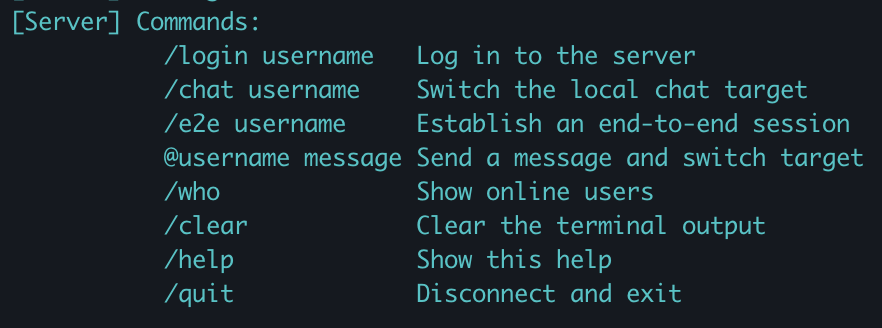
\includegraphics[width=0.75\linewidth]{images/commands.png}
    \caption{Command-line tools inside the chat}
\end{figure}

\begin{figure}[H]
    \centering
    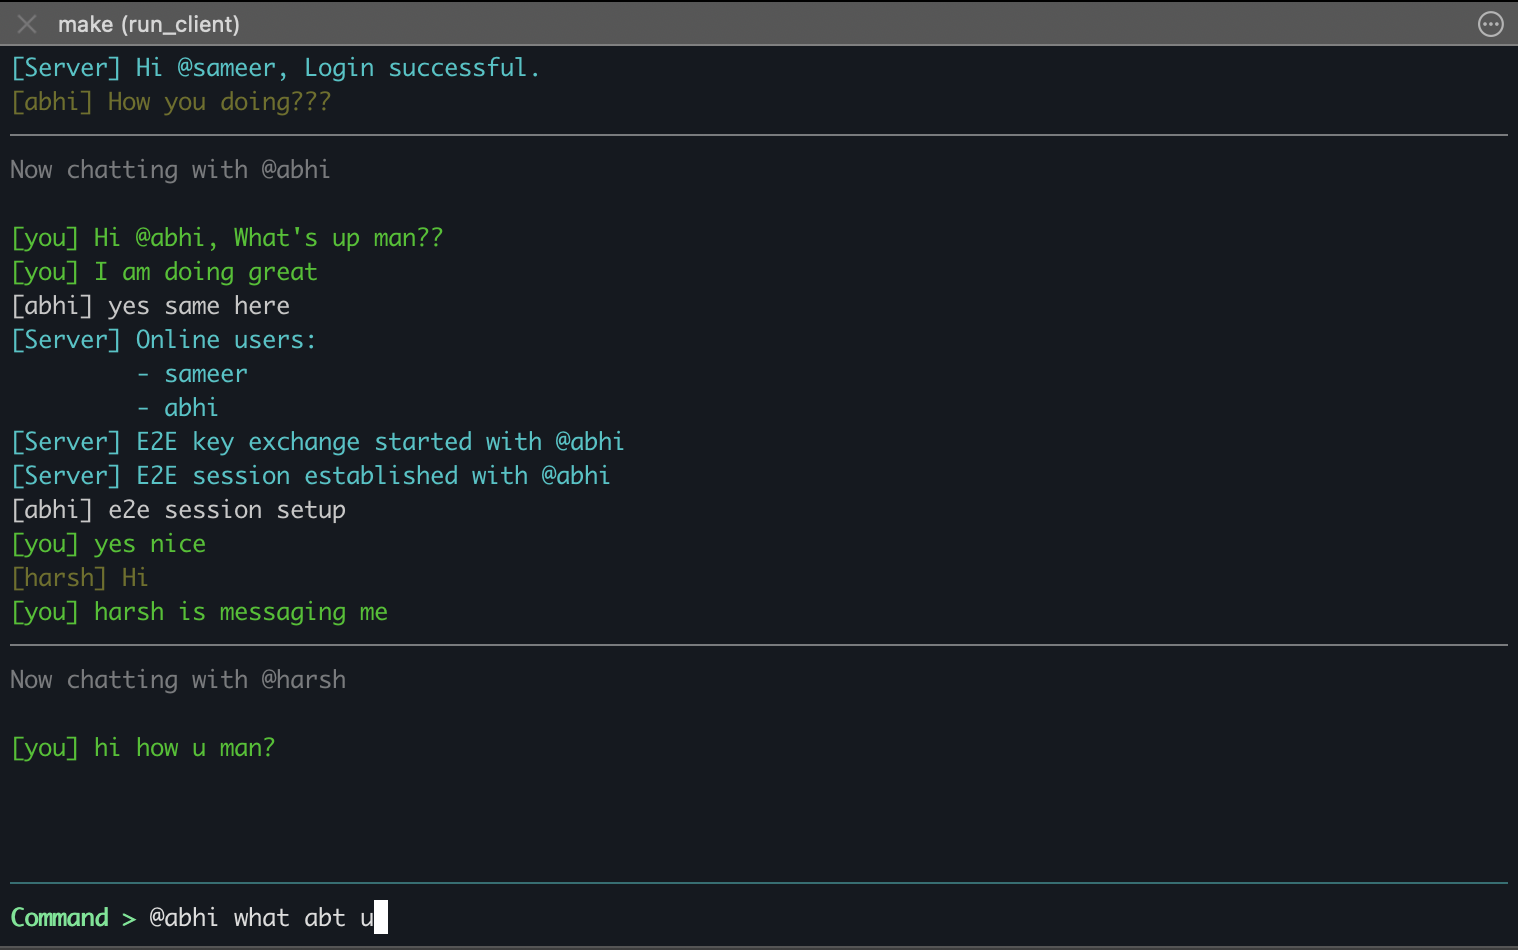
\includegraphics[width=0.75\linewidth]{images/interface.png}
    \caption{Interface of the secure chat application.}
\end{figure}
% =================================================
% PHASE 1
% =================================================
\section{Phase 1 -- Baseline Chat}

\subsection{Implementation}

TCP provides a byte stream rather than message boundaries, so the protocol uses \textbf{length-prefixed framing}: every serialized message is preceded by a 4-byte length field. The receiver first reads the length and then repeatedly calls \texttt{recv()} until exactly that many bytes have been collected. Thus, a message is complete only when its full framed payload has arrived.

The server maintains logged-in users in a username-to-socket registry. Messages such as \texttt{@username message} are routed by looking up the destination username and forwarding the message to that socket. This logic is not tied to exactly two users and can route among any number of registered clients. The required \texttt{/chat}, \texttt{/who}, and \texttt{/quit} commands are also handled by the client/server protocol.

\subsection{Verification}

The server logs each relayed message in plaintext, confirming that in Phase 1 the server can read complete chat contents. Wireshark likewise exposes the plaintext when following the corresponding TCP stream.


\begin{figure}[H]
    \centering
    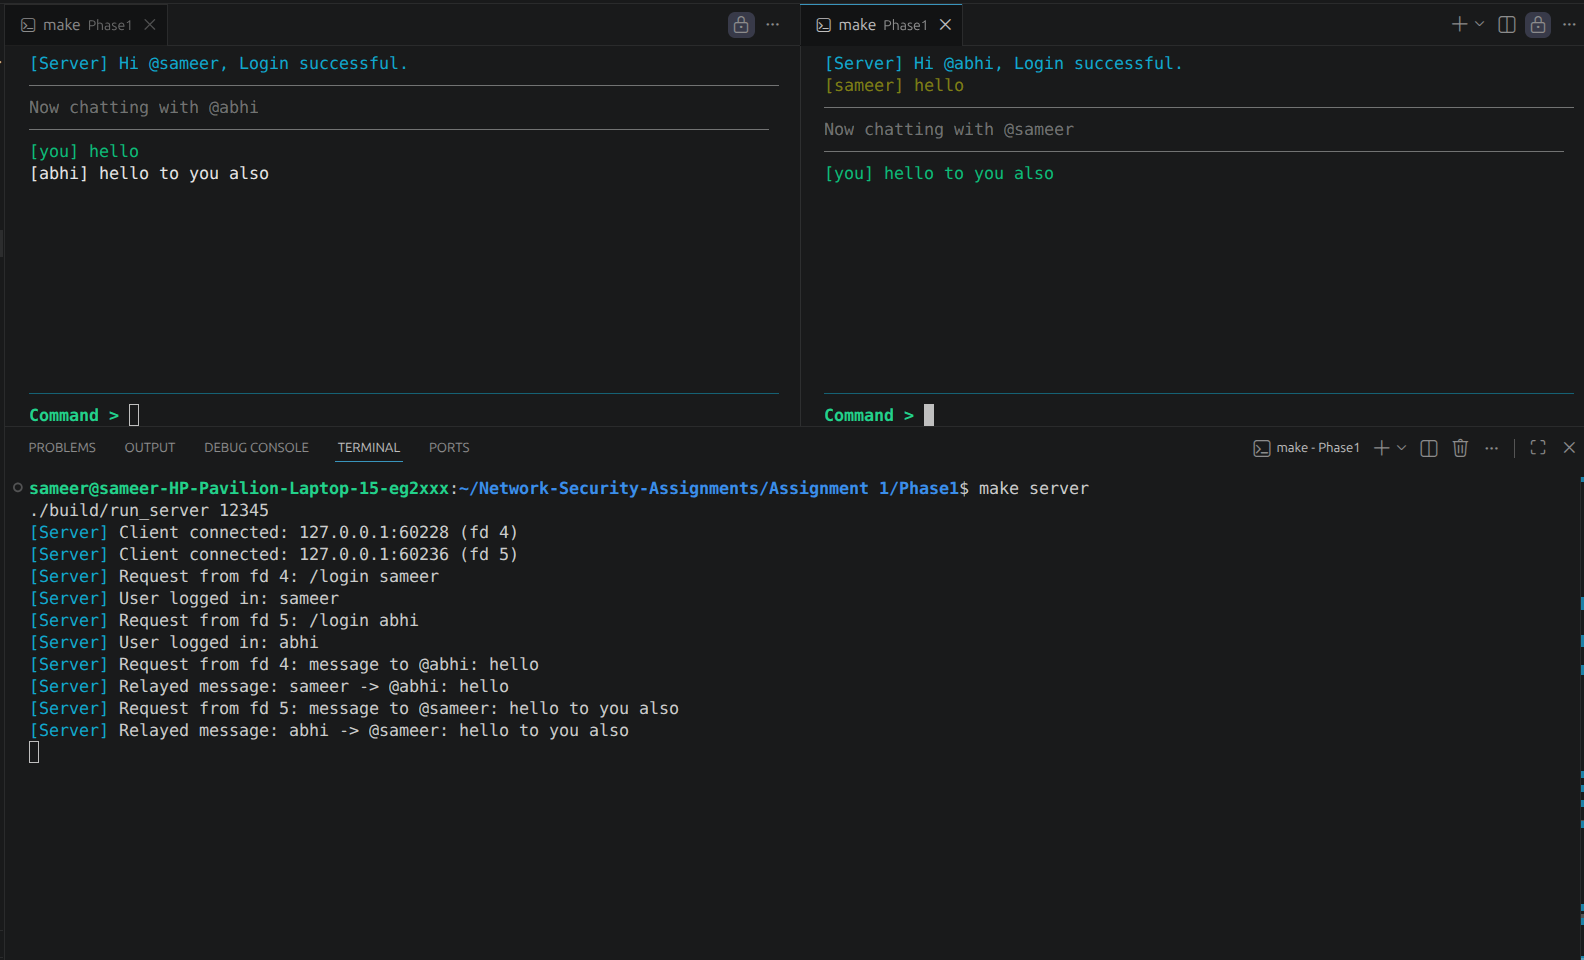
\includegraphics[width=0.90\linewidth]{images/phase1/usage.png}
    \caption{Server can read message contents in Phase 1.}
\end{figure}

\begin{figure}[H]
    \centering
    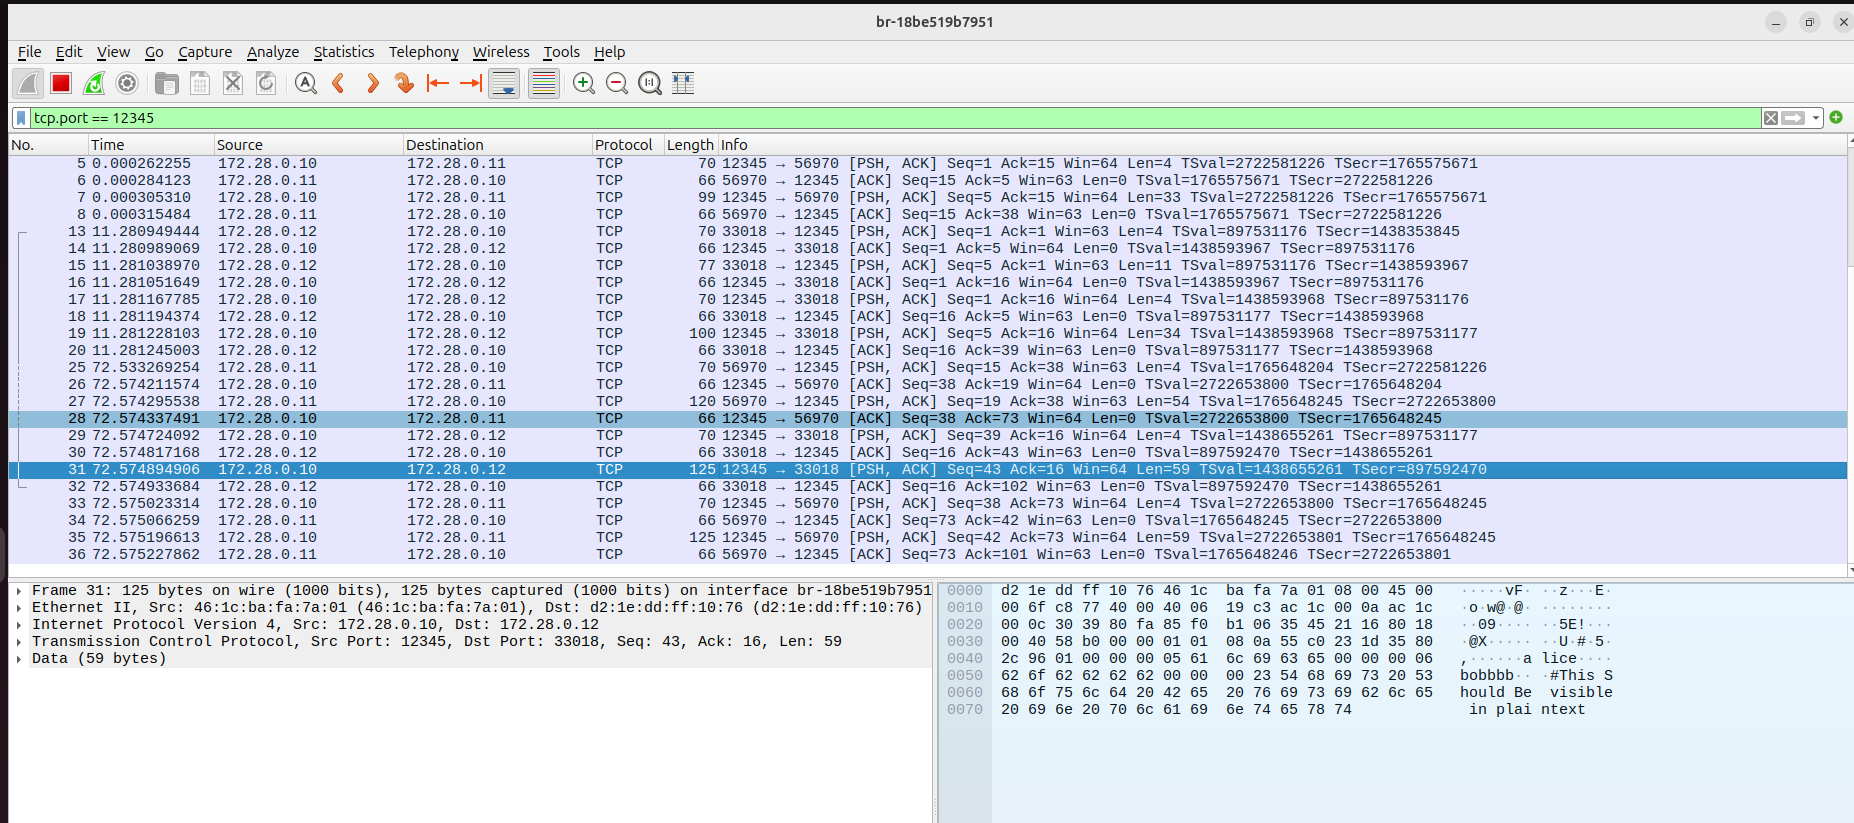
\includegraphics[width=\linewidth]{images/phase1/wireshark.png}
    \caption{Plaintext visible in the Phase 1 packet capture.}
\end{figure}

% =================================================
% PHASE 2
% =================================================
\section{Phase 2 -- Client--Server Confidentiality}

\subsection{DH and AES-GCM Design}

Each client performs an independent Diffie--Hellman exchange with the server. The submitted implementation uses a fixed published MODP-style prime constant (named \texttt{RFC3526\_GROUP14\_PRIME} in the code), generator $g=2$, and implements modular exponentiation directly using square-and-multiply over OpenSSL \texttt{BIGNUM} arithmetic rather than a library DH API.

After computing the DH shared secret $s$, the application derives the 256-bit symmetric key as
\[
K = \mathrm{SHA256}(\mathrm{encode}(s)).
\]
The raw DH value is hashed so that the variable-format group element is converted into a fixed-size, uniformly formatted 256-bit key suitable for AES-256, while avoiding direct use of the raw shared secret as an AES key.

All post-handshake protocol messages are encrypted using AES-256-GCM. Each ciphertext carries the GCM IV/nonce and authentication tag. Therefore, GCM provides both confidentiality and integrity: altered ciphertext fails authentication instead of producing silently corrupted plaintext.

\subsection{Required Verification}

Both endpoints print only a hash-based fingerprint of the derived secret/key material; matching fingerprints demonstrate that the two sides derived the same channel key without revealing the raw secret.

\begin{figure}[H]
\centering
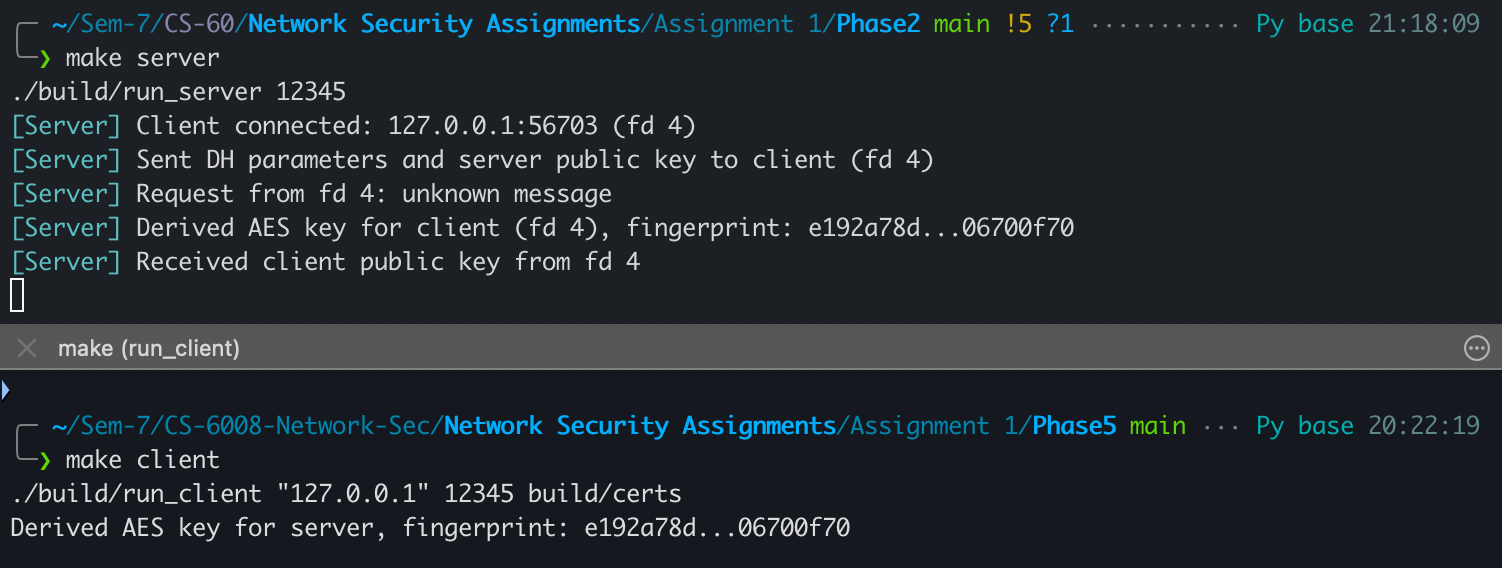
\includegraphics[width=0.80\linewidth]{images/phase2/DH_fingerprints.png}
\caption{Matching key fingerprints at both ends of exchange: Server and Client.}
\end{figure}

\subsection{Wireshark Capture}

Repeating the Phase 1 Wireshark experiment shows framed ciphertext instead of readable chat content.

\begin{figure}[H]
    \centering
    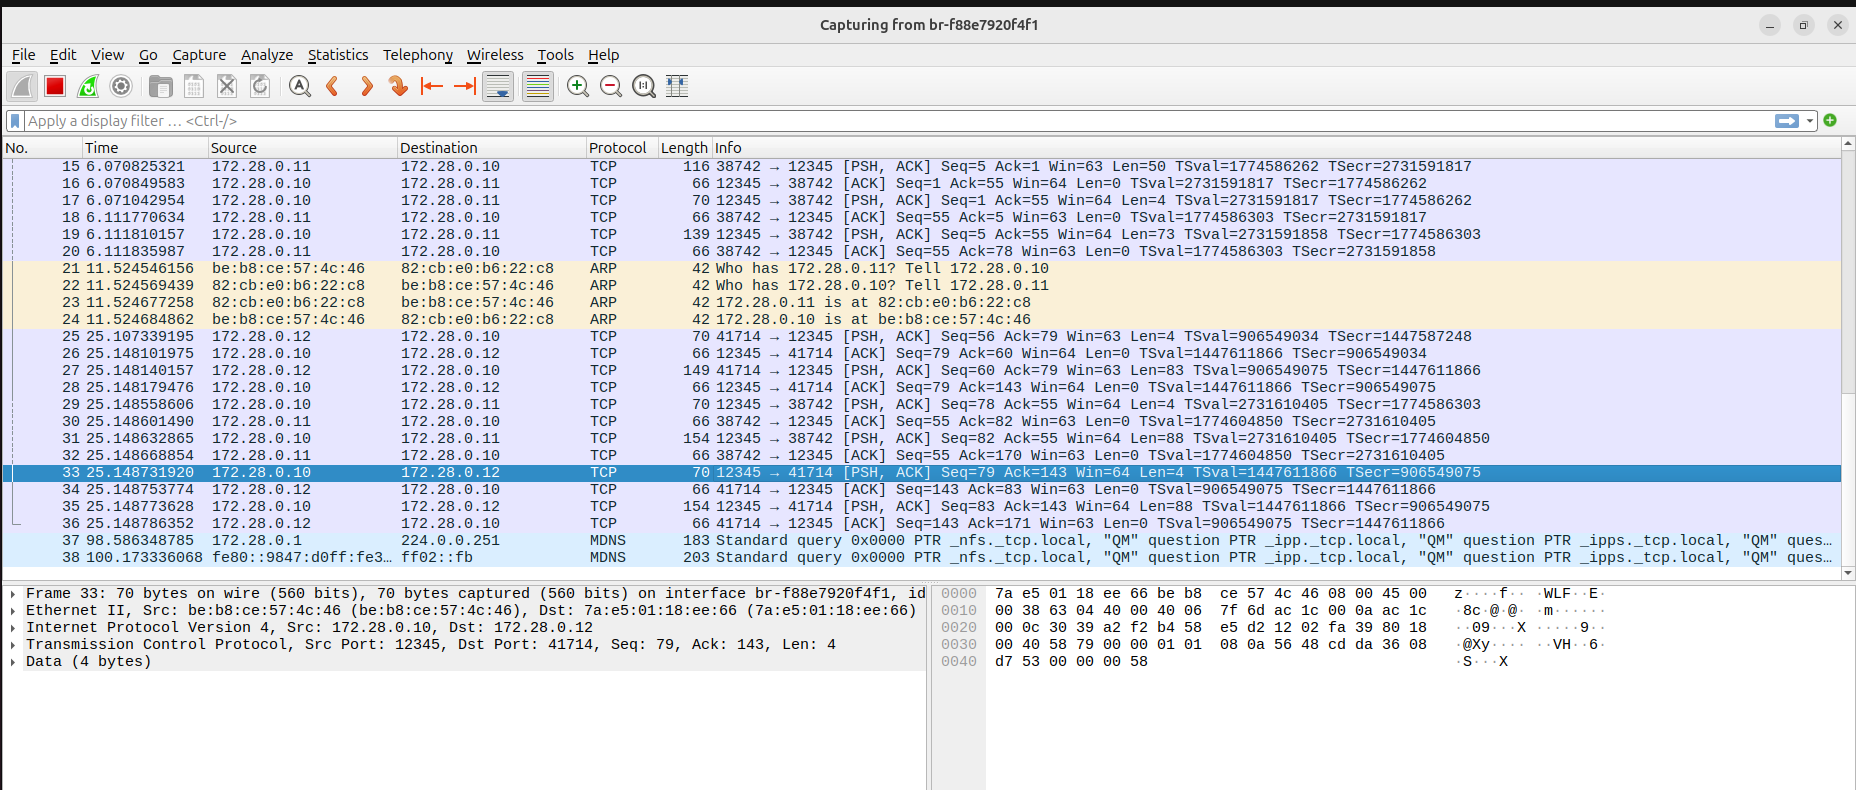
\includegraphics[width=\linewidth]{images/phase2/wireshark.png}
    \caption{Chat content is no longer readable on the client--server link.}
\end{figure}

\subsection{Integrity Test}

For the integrity test, the implementation supports intentionally modifying a ciphertext byte before reception. AES-GCM rejects the modified record because the authentication tag no longer verifies.

\begin{figure}[H]
    \centering
    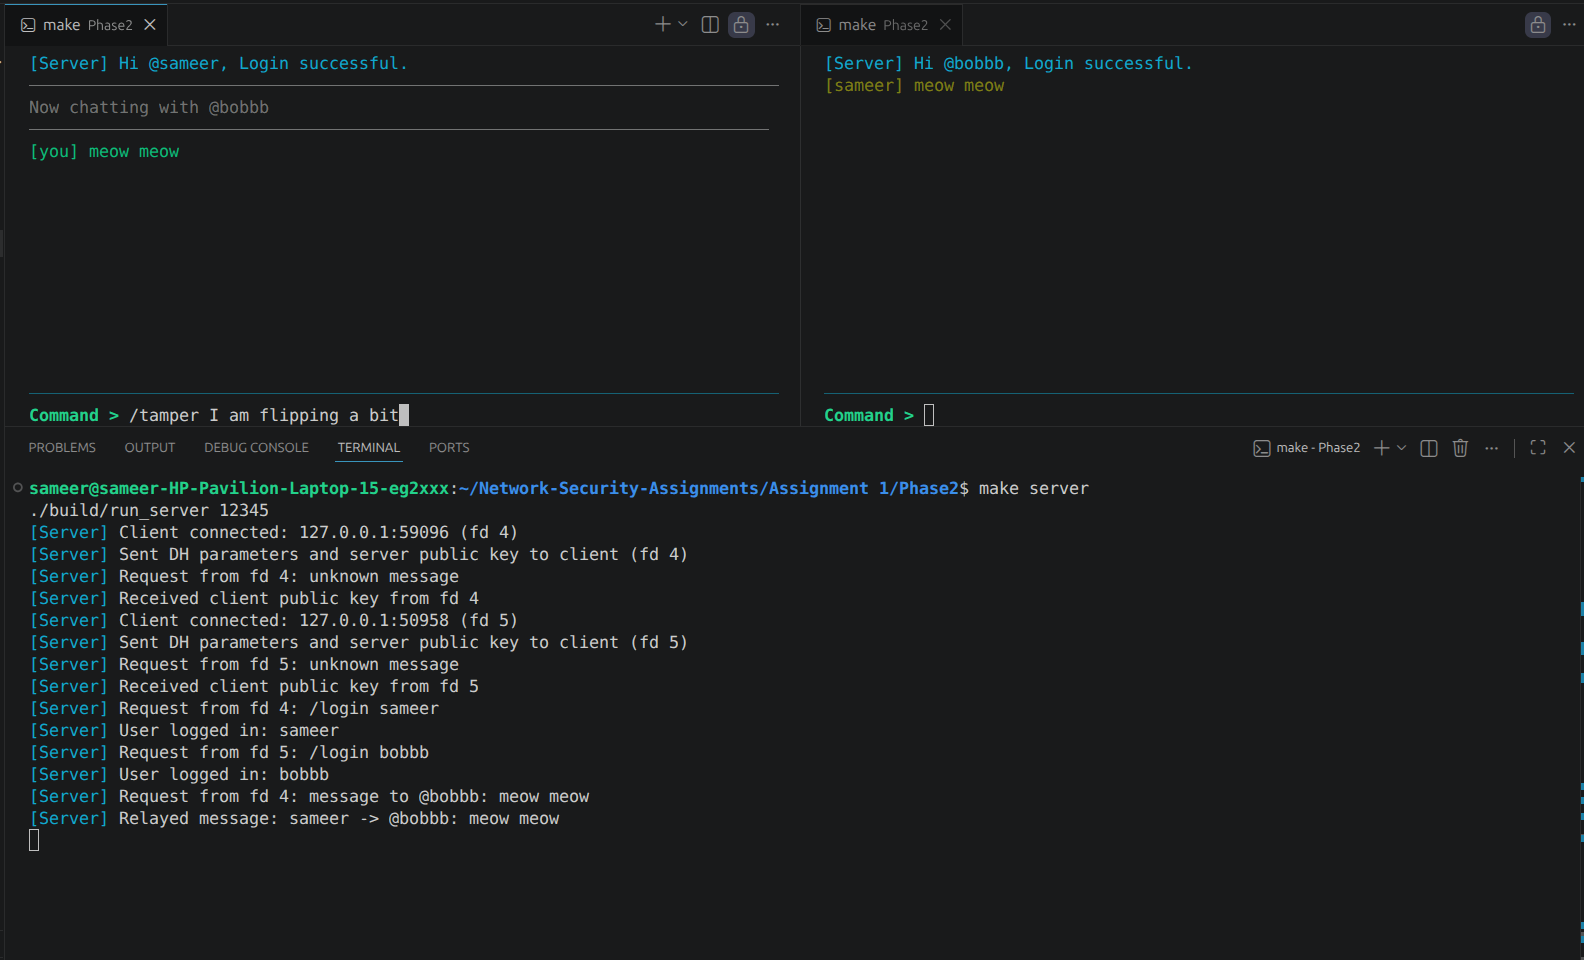
\includegraphics[width=0.75\linewidth]{images/phase2/tamper1.png}
    \caption{Single-byte ciphertext modification attempt using \texttt{/tamper} command.}
\end{figure}
\begin{figure}[H]
\centering
    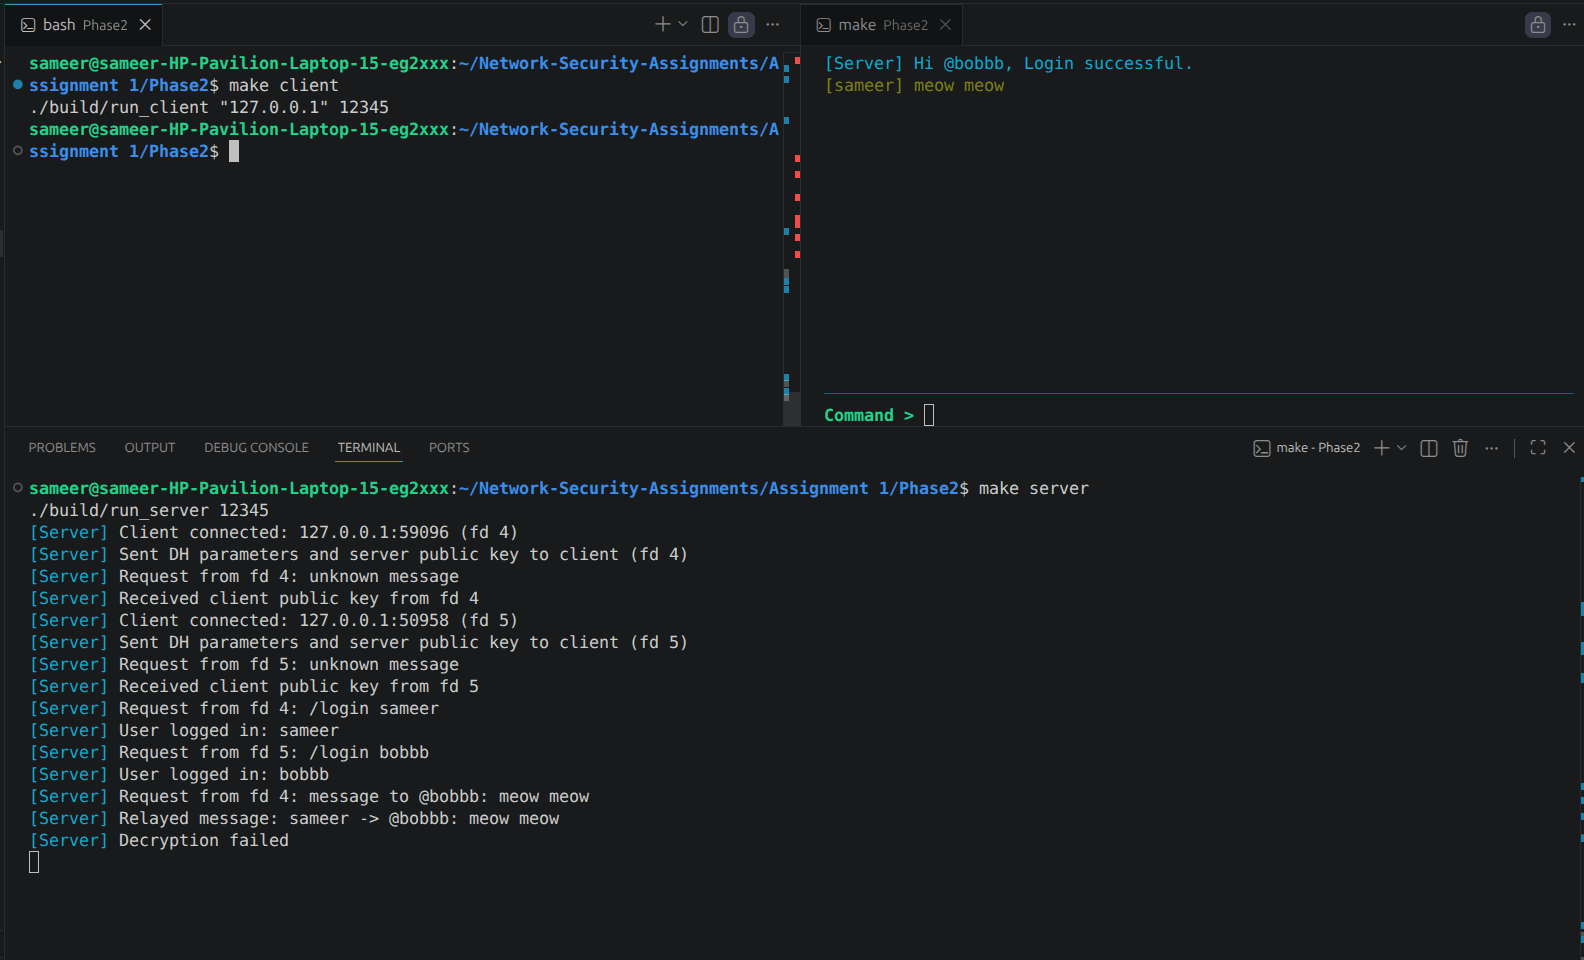
\includegraphics[width=0.75\linewidth]{images/phase2/tamper2.png}
\caption{Phase 2 tamper test attempt showing GCM authentication/decryption failure}
\end{figure}

\subsection{MITM Attack}

The Phase 2 MITM proxy is placed on Mallory between the victim client and the real server. It performs two independent DH exchanges: one while posing as the server to the client and another while posing as the client to the real server. The proxy therefore obtains one AES key for each side, decrypts a received message, logs its plaintext, and re-encrypts it under the key for the other link.

\begin{figure}[H]
\centering
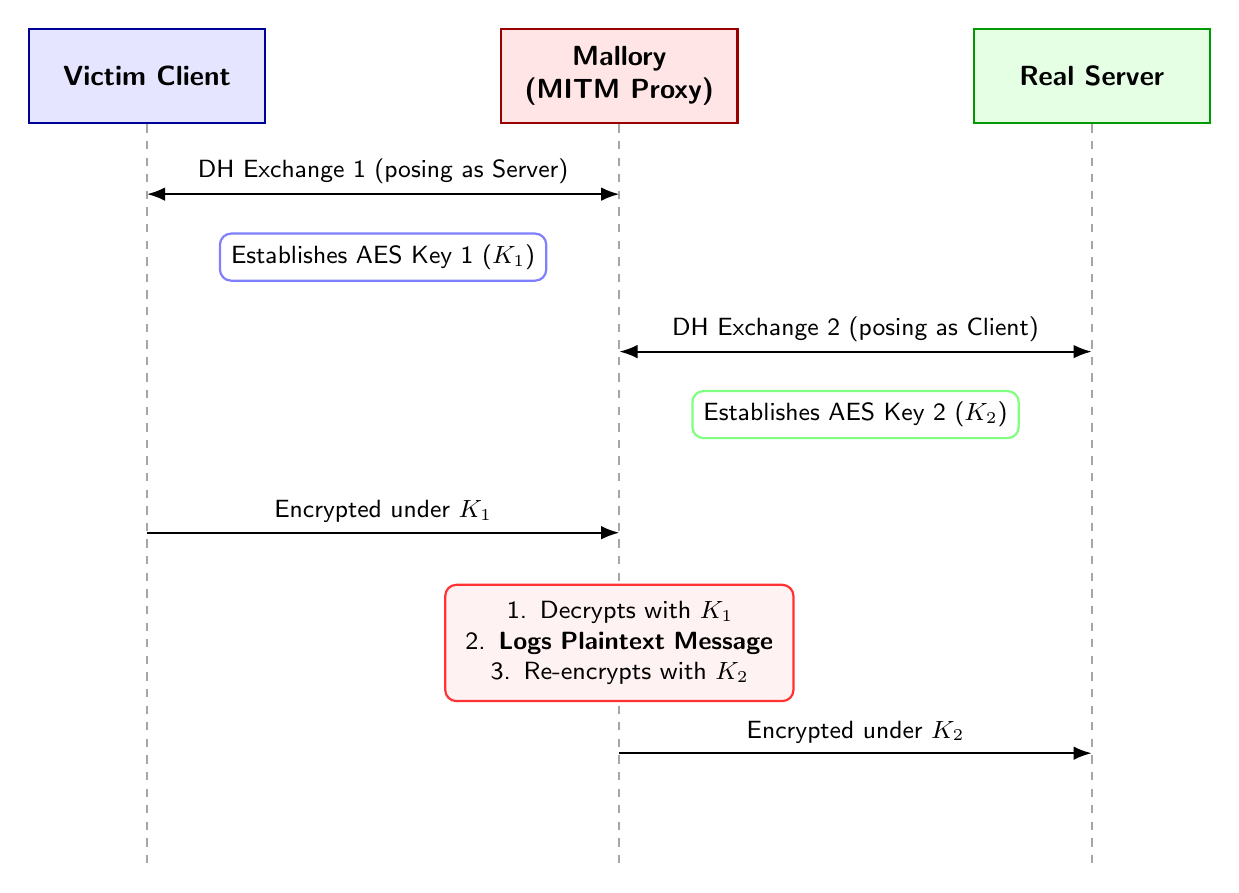
\begin{tikzpicture}[
    >=Latex,
    thick,
    entity/.style={draw, minimum width=3cm, minimum height=1.2cm, fill=gray!10, align=center, font=\sffamily\bfseries},
    client/.style={entity, fill=blue!10, draw=blue!60!black},
    mallory/.style={entity, fill=red!10, draw=red!60!black},
    server/.style={entity, fill=green!10, draw=green!60!black},
    actionbox/.style={draw=red!80, fill=red!5, rounded corners, align=center, text width=4cm, font=\sffamily\small, inner sep=6pt},
    notebox/.style={draw=gray!50, fill=white, rounded corners, font=\sffamily\small, inner sep=4pt}
]

    % Define X coordinates for the lifelines
    \def\clientX{0}
    \def\malloryX{6}
    \def\serverX{12}
    \def\bottomY{-10}

    % Nodes for the entities
    \node[client] (C) at (\clientX, 0) {Victim Client};
    \node[mallory] (M) at (\malloryX, 0) {Mallory\\(MITM Proxy)};
    \node[server]  (S) at (\serverX, 0) {Real Server};

    % Draw Lifelines
    \draw[dashed, draw=gray!70] (C.south) -- (\clientX, \bottomY);
    \draw[dashed, draw=gray!70] (M.south) -- (\malloryX, \bottomY);
    \draw[dashed, draw=gray!70] (S.south) -- (\serverX, \bottomY);

    % ---------------------------------------------------------
    % DH Exchange 1: Client <--> Mallory
    % ---------------------------------------------------------
    \draw[<->] (\clientX, -1.5) -- (\malloryX, -1.5) 
        node[midway, above, font=\sffamily\small] {DH Exchange 1 (posing as Server)};
    
    \node[notebox, draw=blue!50] at ($(\clientX, -2.3)!0.5!(\malloryX, -2.3)$) {Establishes AES Key 1 ($K_1$)};

    % ---------------------------------------------------------
    % DH Exchange 2: Mallory <--> Server
    % ---------------------------------------------------------
    \draw[<->] (\malloryX, -3.5) -- (\serverX, -3.5) 
        node[midway, above, font=\sffamily\small] {DH Exchange 2 (posing as Client)};
    
    \node[notebox, draw=green!50] at ($(\malloryX, -4.3)!0.5!(\serverX, -4.3)$) {Establishes AES Key 2 ($K_2$)};

    % ---------------------------------------------------------
    % Message Forwarding & Interception
    % ---------------------------------------------------------
    % 1. Client sends encrypted message to Mallory
    \draw[->] (\clientX, -5.8) -- (\malloryX, -5.8) 
        node[midway, above, font=\sffamily\small] {Encrypted under $K_1$};

    % 2. Mallory intercepts, decrypts, logs, re-encrypts
    \node[actionbox] at (\malloryX, -7.2) {
        1. Decrypts with $K_1$\\
        2. \textbf{Logs Plaintext Message}\\
        3. Re-encrypts with $K_2$
    };

    % 3. Mallory sends newly encrypted message to Server
    \draw[->] (\malloryX, -8.6) -- (\serverX, -8.6) 
        node[midway, above, font=\sffamily\small] {Encrypted under $K_2$};

\end{tikzpicture}
\caption{Explaining the Phase 2 MITM proxy attack: Mallory establishes two independent DH/AES channels, decrypts and logs messages, and forwards them without alerting the client or server.}
\end{figure}

\begin{figure}[H]
\centering
    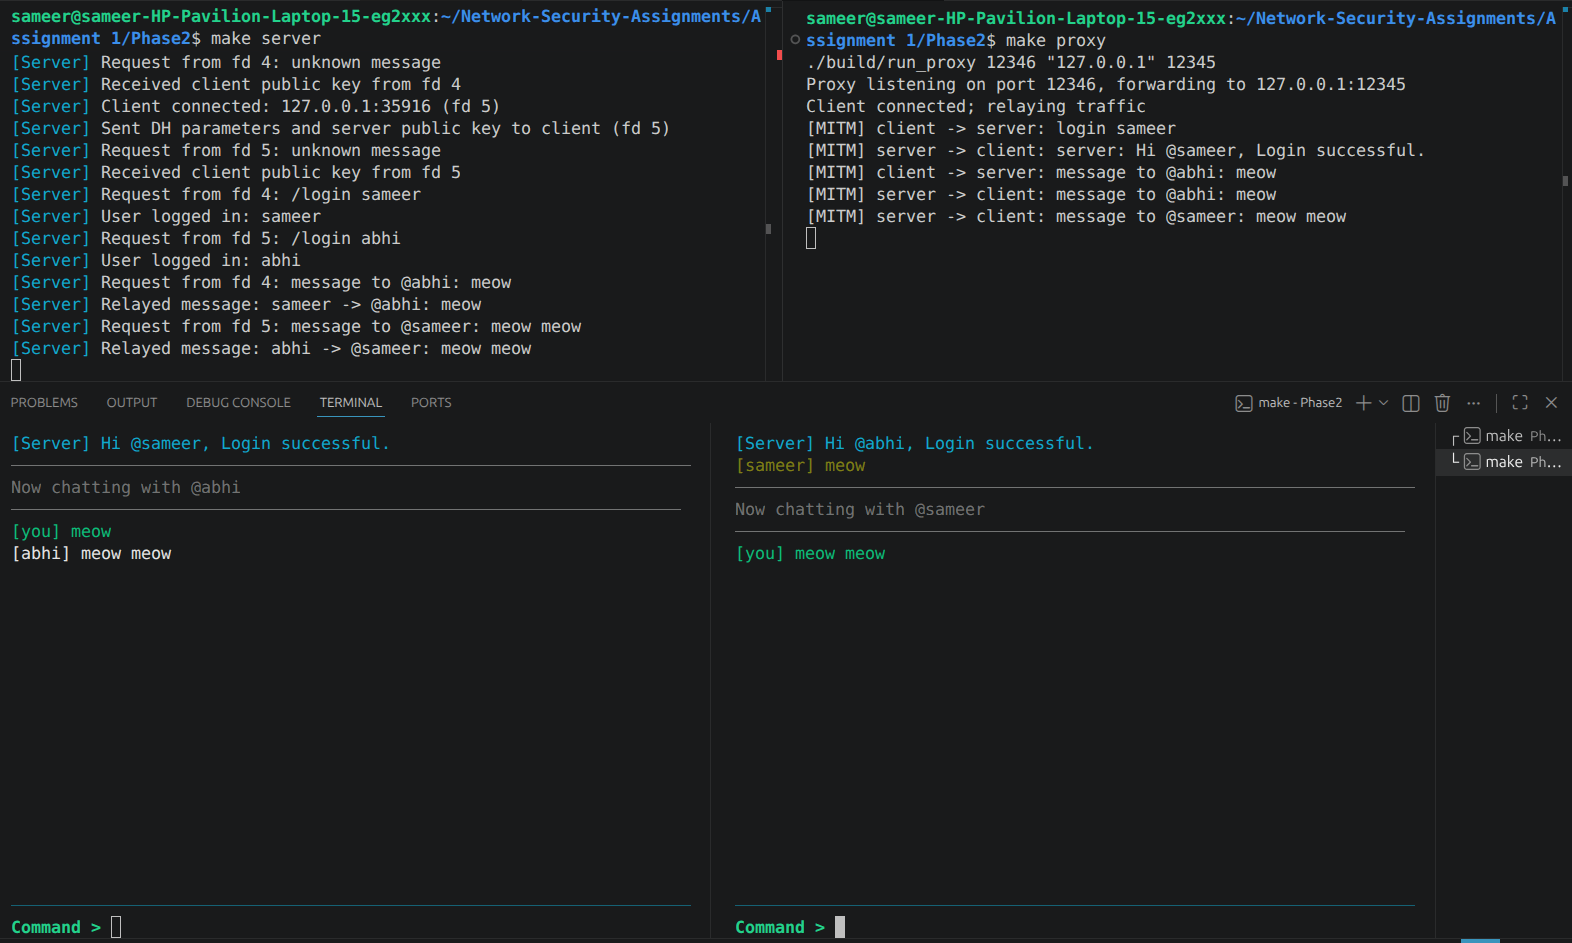
\includegraphics[width=\linewidth]{images/phase2/proxy_use.png}
    \caption{Demonstration of the Phase 2 Man-in-the-Middle proxy attack. The proxy (top right) successfully intercepts, decrypts, and logs the plaintext communications between the chat server (top left) and the victim client (bottom left pane) without alerting the users.}
% \caption{Phase 2 tamper test showing GCM authentication/decryption failure}
\end{figure}

The main observable indication is that the client and real server do \emph{not} share the same DH fingerprint with each other: each instead shares a different key with Mallory. However, without an authenticated reference fingerprint or authenticated server identity, an ordinary user has no trusted value against which to compare the result. The connection still functions normally, so the attack is unlikely to be noticed from the chat interface alone.

% =================================================
% PHASE 3
% =================================================
\section{Phase 3 -- Server Authentication via PKI}

\subsection{PKI Setup}

A private CA and CA-signed server certificate are generated with OpenSSL. The server certificate uses identity \texttt{chat-server}, including \texttt{subjectAltName = DNS:chat-server}. The client stores only the trusted CA certificate; the CA private key is not distributed.

The implemented certificate-generation flow is summarized below:

\begin{lstlisting}[basicstyle=\ttfamily\small,breaklines=true]
openssl genrsa -out ca.key 4096
openssl req -x509 -new -key ca.key -sha256 -days 3650 \
  -out ca.crt \
  -subj "/C=IN/ST=Maharashtra/L=Mumbai/O=MyChat/OU=CA/CN=MyChat Root CA"

openssl genrsa -out server.key 2048
openssl req -new -key server.key -out server.csr \
  -subj "/C=IN/ST=Maharashtra/L=Mumbai/O=MyChat/OU=Server/CN=chat-server"

# server-ext.cnf contains:
# subjectAltName = DNS:chat-server
# extendedKeyUsage = serverAuth

openssl x509 -req -in server.csr -CA ca.crt -CAkey ca.key \
  -CAcreateserial -out server.crt -days 365 -sha256 \
  -extfile server-ext.cnf

openssl verify -CAfile ca.crt server.crt
\end{lstlisting}

\subsection{Authenticated Handshake Design}

Before DH key establishment, the server sends its certificate. The client builds a trust store containing its local \texttt{ca.crt} and verifies the certificate chain/signature and validity through X.509 verification. It then checks the expected server identity \texttt{chat-server} using hostname validation. If any certificate check fails, the connection is aborted before the DH exchange or application login proceeds.

A valid certificate alone is insufficient because an attacker could copy \texttt{server.crt}. The server must also prove possession of the matching private key. The client sends a fresh challenge $R$ together with its DH public value $A$. The server chooses its DH public value $B$ and signs the transcript
\[
\texttt{``MYCHAT-HANDSHAKE-V1''} \parallel R \parallel A \parallel B.
\]
The client verifies this signature with the public key extracted from the validated server certificate. Only then does it derive the DH/AES key. Binding $R$, $A$, and $B$ to the signature also makes the proof specific to the current handshake.

\begin{figure}[H]
\centering
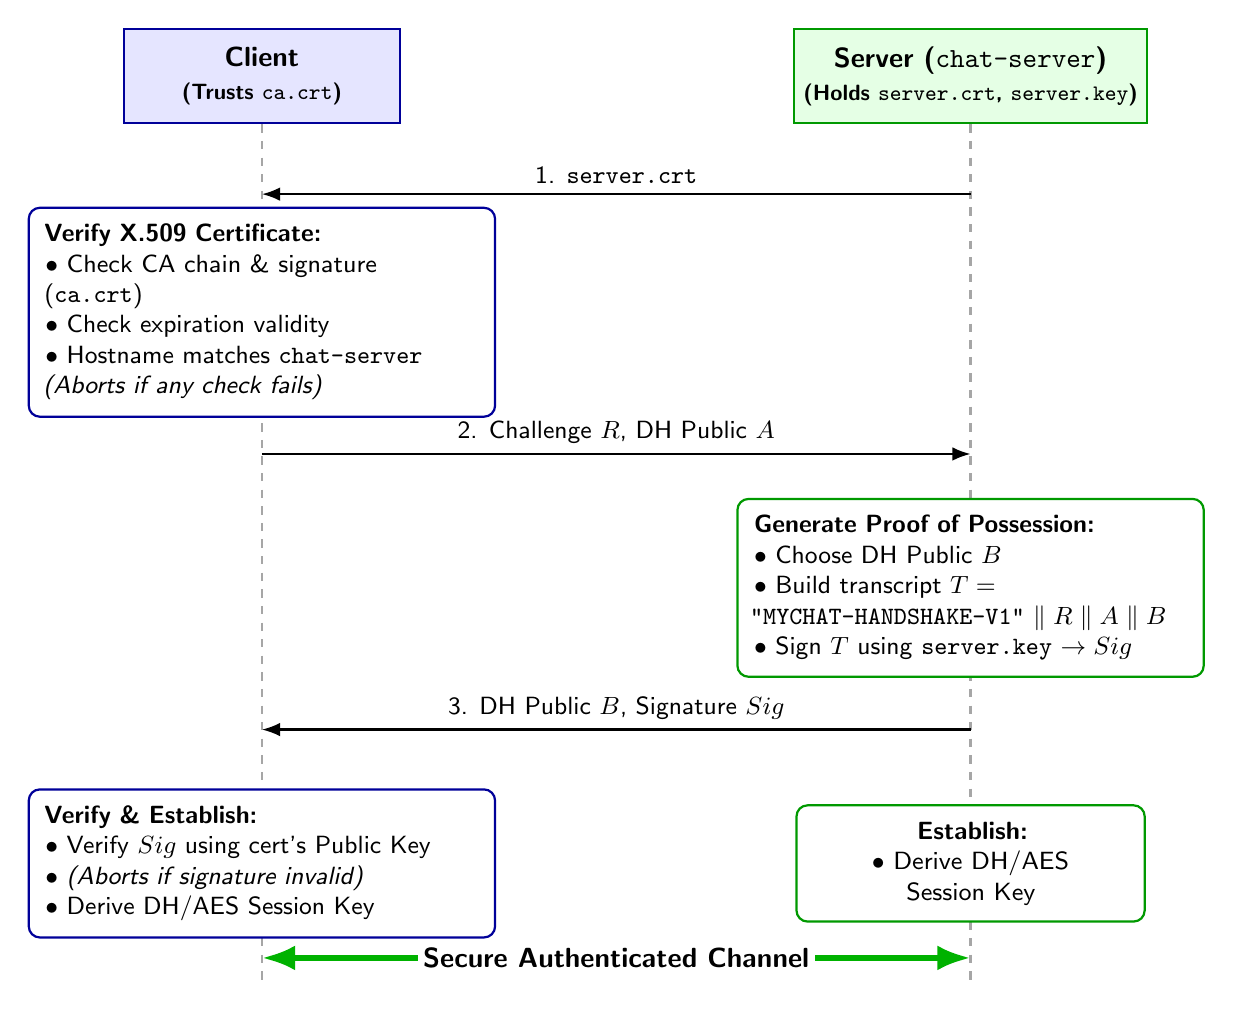
\begin{tikzpicture}[
    >=Latex,
    thick,
    entity/.style={draw, minimum width=3.5cm, minimum height=1.2cm, fill=gray!10, align=center, font=\sffamily\bfseries},
    client/.style={entity, fill=blue!10, draw=blue!60!black},
    server/.style={entity, fill=green!10, draw=green!60!black},
    actionbox/.style={draw=gray!80, fill=white, rounded corners, align=left, text width=5.5cm, font=\sffamily\small, inner sep=6pt},
    notebox/.style={draw=yellow!60!black, fill=yellow!10, rounded corners, font=\sffamily\footnotesize, inner sep=4pt}
]

    % Define X coordinates for the lifelines
    \def\clientX{0}
    \def\serverX{9}
    \def\bottomY{-11.5}

    % Nodes for the entities
    \node[client] (C) at (\clientX, 0) {Client\\{\footnotesize (Trusts \texttt{ca.crt})}};
    \node[server] (S) at (\serverX, 0) {Server (\texttt{chat-server})\\{\footnotesize (Holds \texttt{server.crt}, \texttt{server.key})}};

    % Draw Lifelines
    \draw[dashed, draw=gray!70] (C.south) -- (\clientX, \bottomY);
    \draw[dashed, draw=gray!70] (S.south) -- (\serverX, \bottomY);

    % 1. Server sends certificate
    \draw[<-] (\clientX, -1.5) -- (\serverX, -1.5) 
        node[midway, above, font=\sffamily\small] {1. \texttt{server.crt}};

    % 2. Client verifies certificate
    \node[actionbox, draw=blue!60!black] at (\clientX, -3.0) {
        \textbf{Verify X.509 Certificate:}\\
        $\bullet$ Check CA chain \& signature (\texttt{ca.crt})\\
        $\bullet$ Check expiration validity\\
        $\bullet$ Hostname matches \texttt{chat-server}\\
        \textit{(Aborts if any check fails)}
    };

    % 3. Client sends Challenge and DH Pub A
    \draw[->] (\clientX, -4.8) -- (\serverX, -4.8) 
        node[midway, above, font=\sffamily\small] {2. Challenge $R$, DH Public $A$};

    % 4. Server computes DH Pub B and signs transcript
    \node[actionbox, draw=green!60!black] at (\serverX, -6.5) {
        \textbf{Generate Proof of Possession:}\\
        $\bullet$ Choose DH Public $B$\\
        $\bullet$ Build transcript $T =$\\
          \texttt{"MYCHAT-HANDSHAKE-V1"} $\parallel R \parallel A \parallel B$\\
        $\bullet$ Sign $T$ using \texttt{server.key} $\rightarrow Sig$
    };

    % 5. Server sends B and Signature
    \draw[<-] (\clientX, -8.3) -- (\serverX, -8.3) 
        node[midway, above, font=\sffamily\small] {3. DH Public $B$, Signature $Sig$};

    % 6. Client verifies signature and derives key
    \node[actionbox, draw=blue!60!black] at (\clientX, -10.0) {
        \textbf{Verify \& Establish:}\\
        $\bullet$ Verify $Sig$ using cert's Public Key\\
        $\bullet$ \textit{(Aborts if signature invalid)}\\
        $\bullet$ Derive DH/AES Session Key
    };

    % 7. Server derives key
    \node[actionbox, draw=green!60!black, text width=4cm, align=center] at (\serverX, -10.0) {
        \textbf{Establish:}\\
        $\bullet$ Derive DH/AES Session Key
    };

    % Final Secure Channel indicator
    \draw[<->, line width=2pt, draw=green!70!black] (\clientX, -11.2) -- (\serverX, -11.2) 
        node[midway, fill=white, font=\sffamily\bfseries, inner sep=2pt] {Secure Authenticated Channel};

\end{tikzpicture}
\caption{The Phase 3 authenticated handshake: the client verifies the server's certificate and proof of possession before establishing a secure channel.}
\end{figure}

\begin{figure}[H]
    \centering
    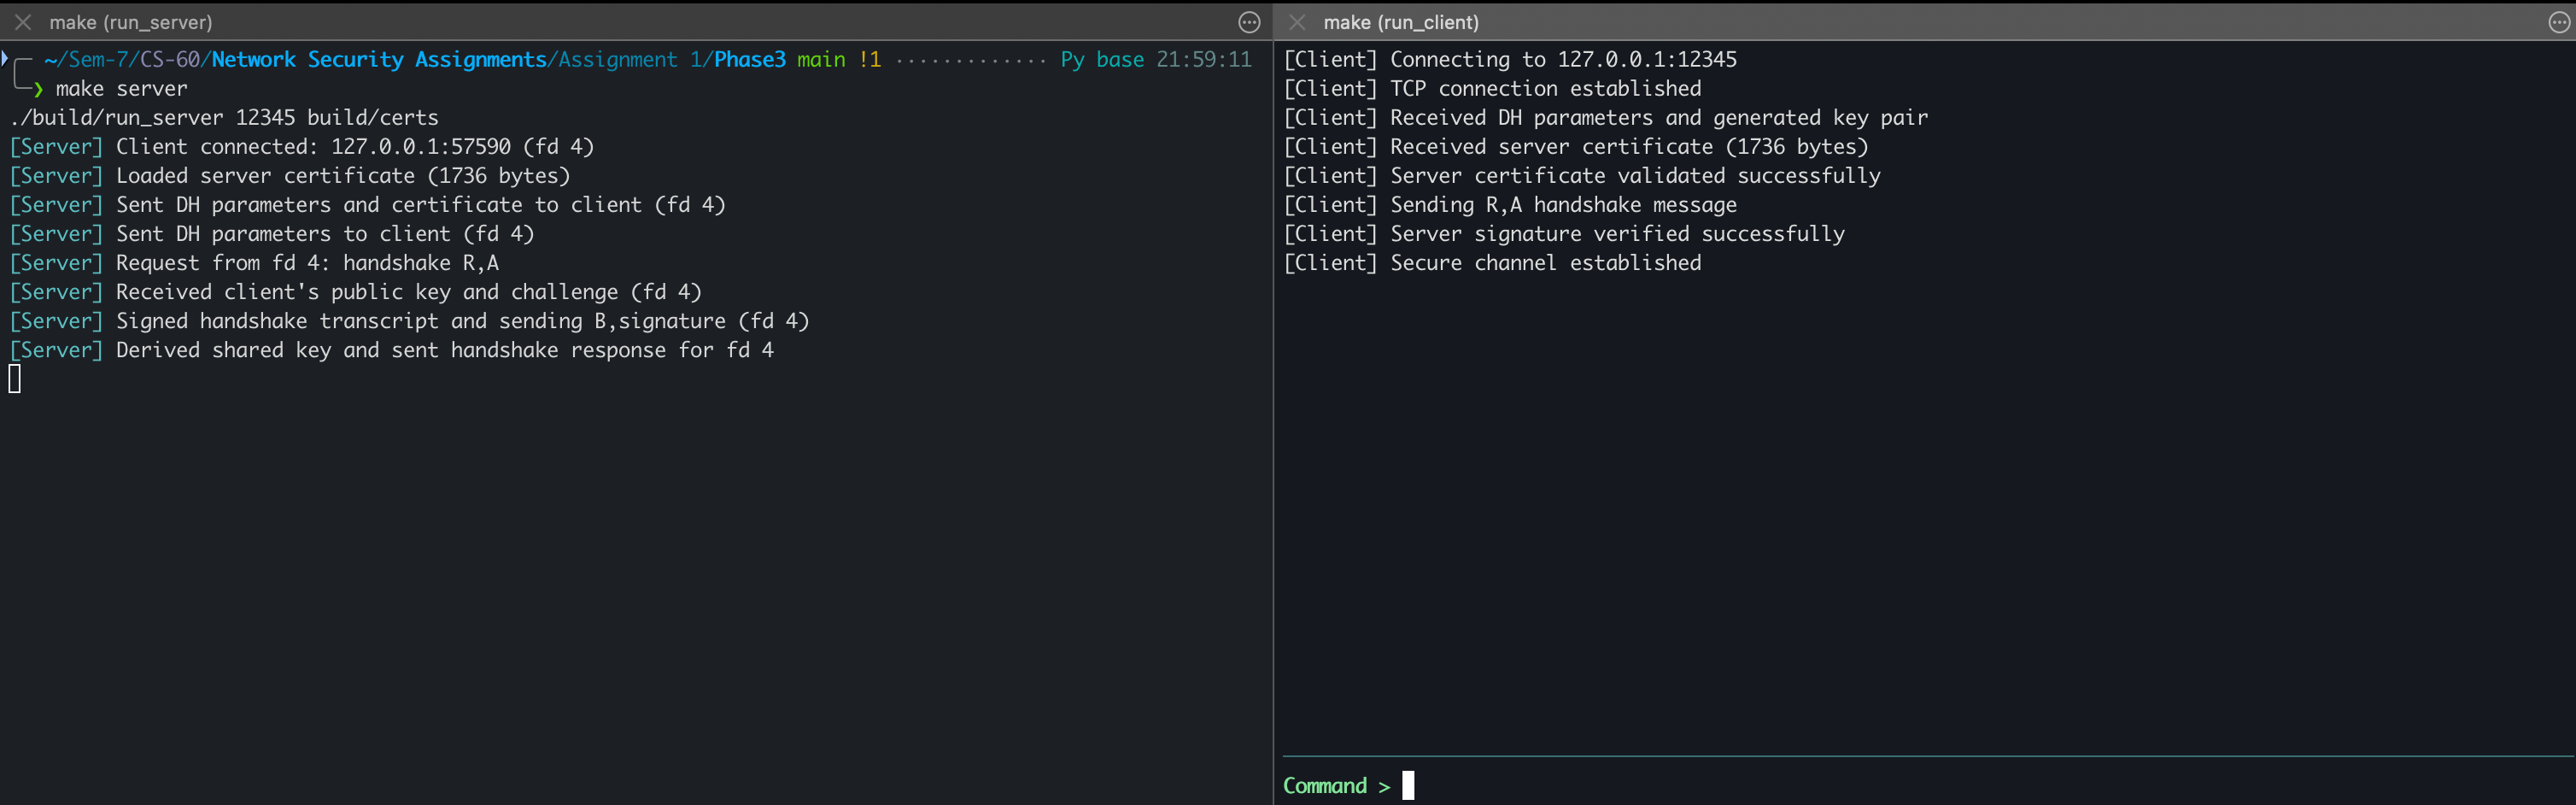
\includegraphics[width=\linewidth]{images/phase3/legitimate.png}
    \caption{Legitimate handshake: connection is established successfully. (Client on right, Server on left)}
\end{figure}

\subsection{Verification and Proxy Re-attempts}

Three proxy modes are present in the Phase 3 implementation. For each mode, three independent runs are recorded below as requested.

\subsubsection*{Phase-2 proxy}
Since here the proxy has no certificate, it cannot even attempt a MITM. The client aborts the connection before any DH exchange.

\begin{figure}[H]
    \centering
    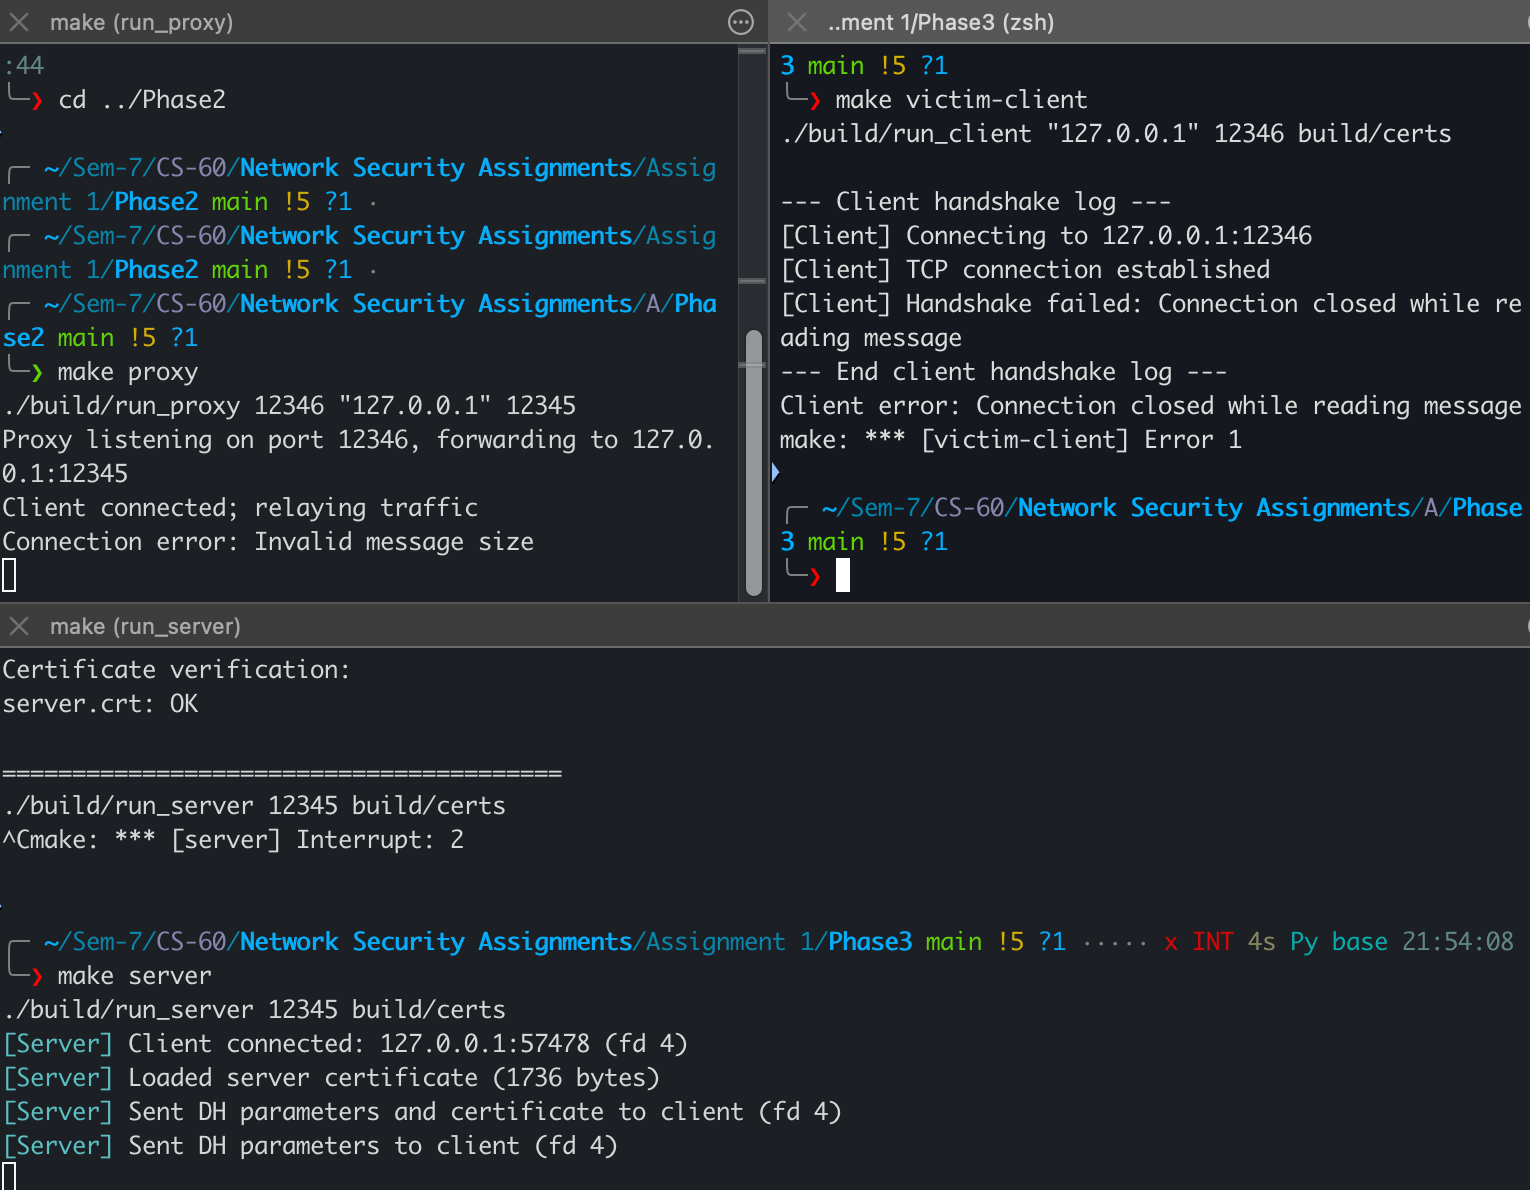
\includegraphics[width=0.60\linewidth]{images/phase3/phase2-proxy.png}
    \caption{Phase-2 proxy: connection is aborted before any DH exchange. (Proxy on top-left, Victim-Client on top-right, Real-Server on bottom)}
\end{figure}

\subsubsection*{Normal proxy -- legitimate authenticated flow}

In \texttt{normal} mode Mallory only forwards raw framed traffic. The genuine server certificate and genuine proof-of-possession signature reach the client unchanged, so certificate validation, signature verification, and DH establishment succeed. The proxy has no session key and cannot inspect encrypted application contents. It only relays opaque ciphertext between the client and server.

\begin{figure}[H]
    \centering
    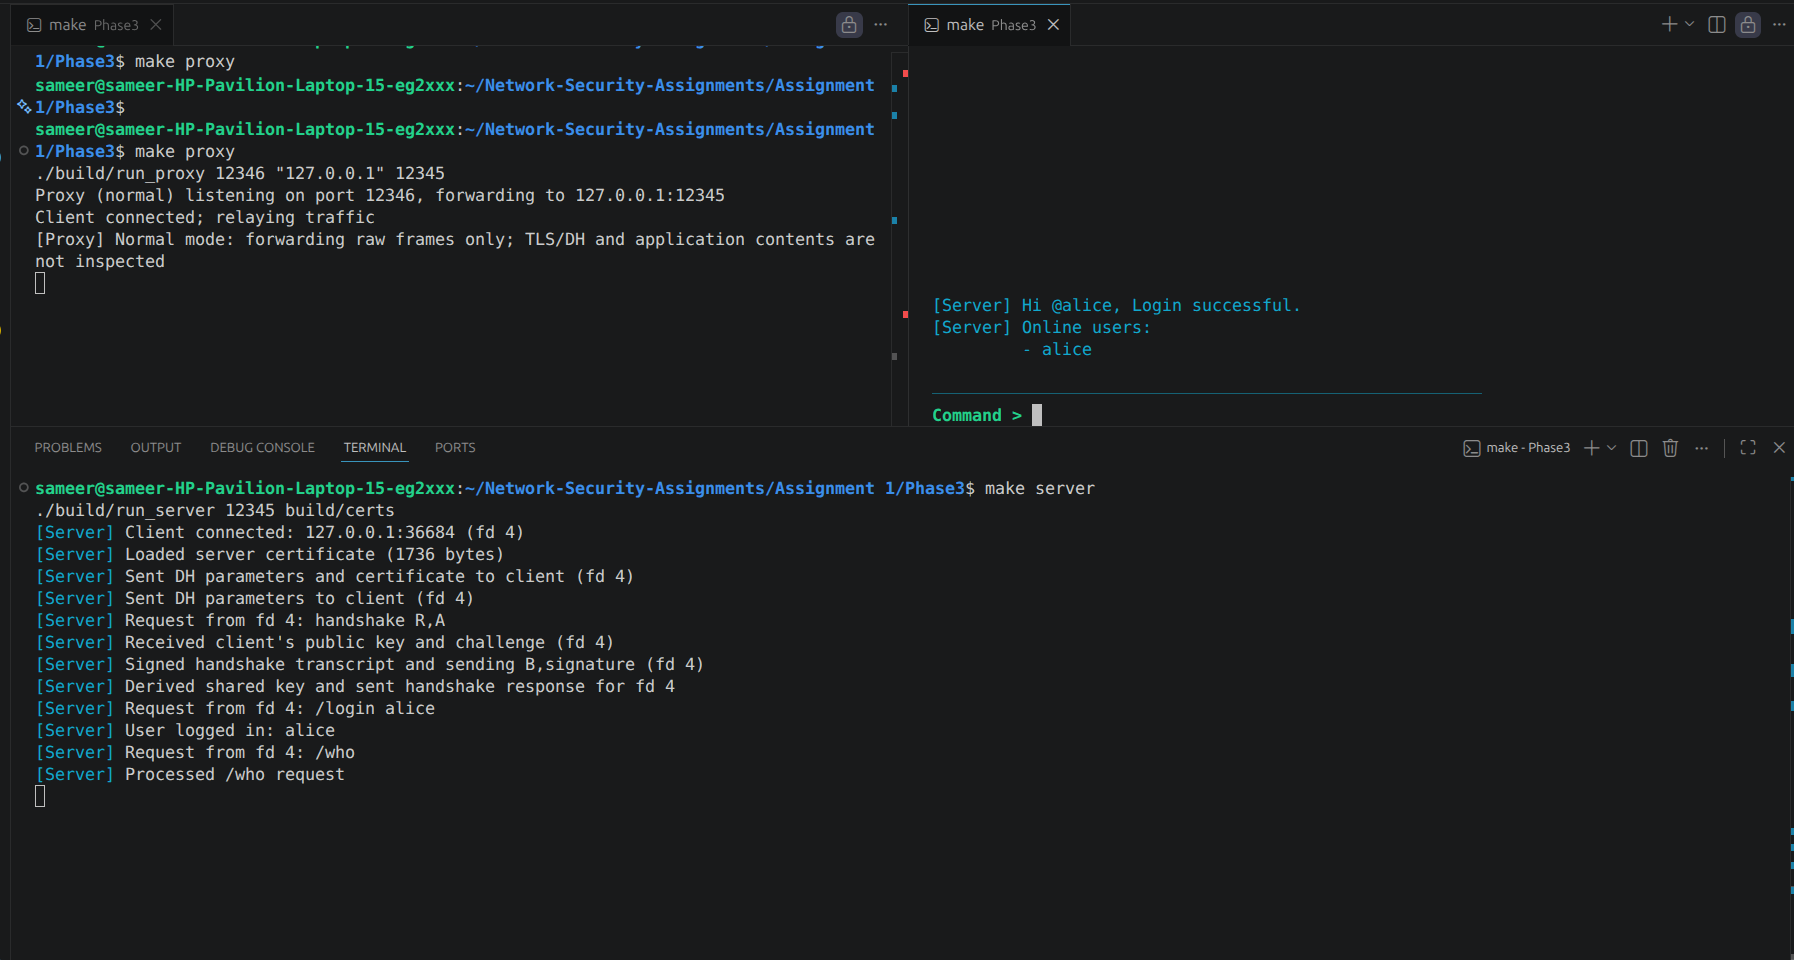
\includegraphics[width=0.75\linewidth]{images/phase3/normal-proxy.png}
    \caption{Normal proxy: legitimate Phase 3 handshake succeeds while Mallory only relays opaque traffic. (Proxy on top-left, Victim-Client on top-right, Real-Server on bottom)}
\end{figure}

\subsubsection*{Fake-certificate proxy -- invalid CA chain}

In \texttt{fake} mode the proxy attempts an active MITM using its own certificate/private-key pair. Although it can create a proof for its own key, its certificate is not signed by the CA trusted by the victim. The client therefore fails certificate validation and aborts before establishing a DH channel with Mallory. This directly contrasts with Phase 2, where the same split-DH strategy succeeded because no server authentication existed through a trusted CA.

\begin{figure}[H]
    \centering
    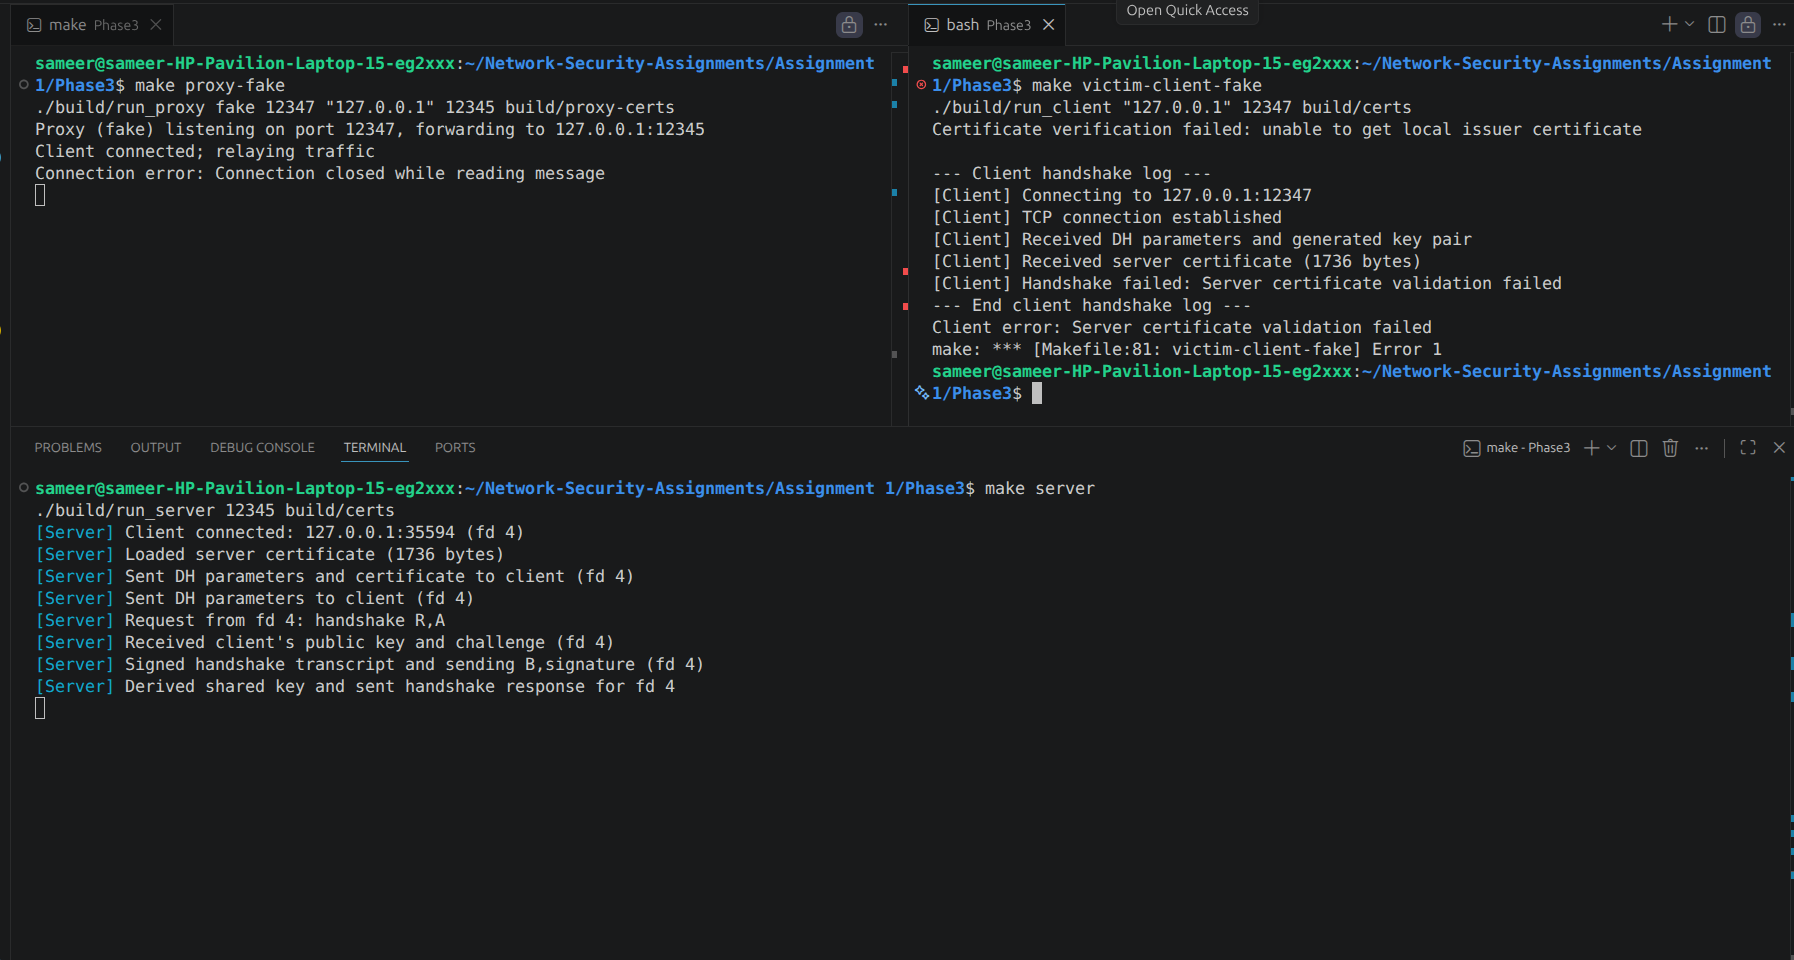
\includegraphics[width=0.75\linewidth]{images/phase3/fake-proxy.png}
    \caption{Fake-certificate MITM is stopped by CA-based certificate validation.\\ (Proxy on top-left, Victim-Client on top-right, Real-Server on bottom)}
\end{figure}

\subsubsection*{Stolen-certificate proxy -- no private key}

In \texttt{thief} mode Mallory forwards/presents the genuine server certificate but does not possess \texttt{server.key}. The certificate can therefore pass CA and hostname checks, but Mallory cannot create the required signature over the fresh $R,A,B$ transcript. The handshake cannot complete and the client does not establish an authenticated channel with the attacker.

\begin{figure}[H]
    \centering
    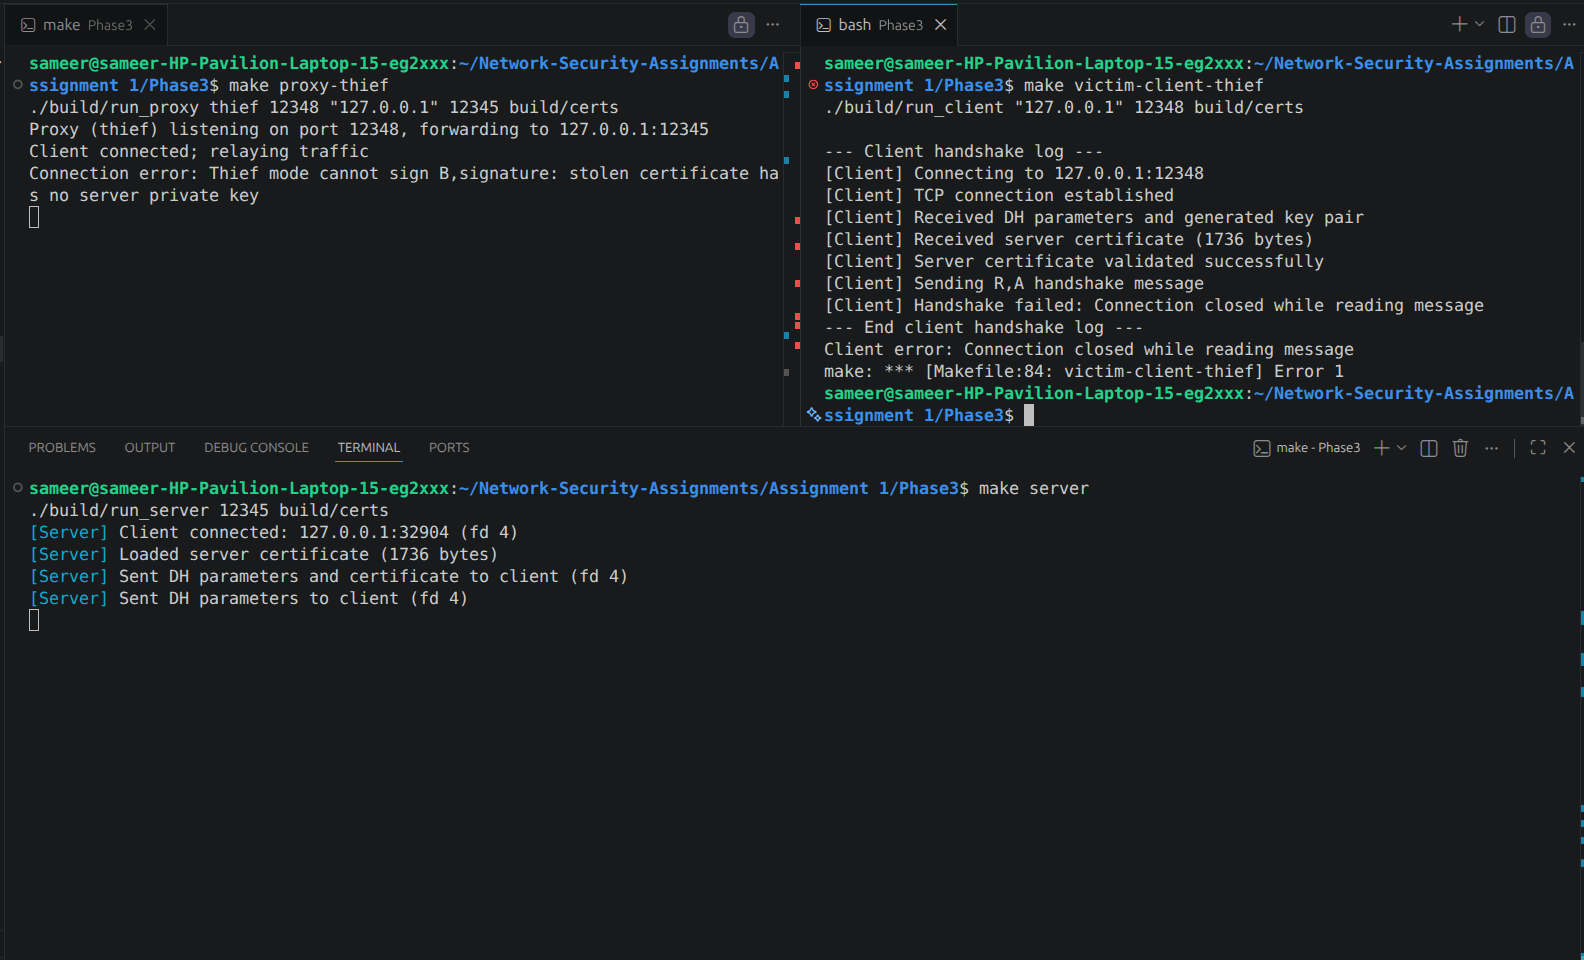
\includegraphics[width=0.75\linewidth]{images/phase3/thief-proxy.png}
    \caption{A copied certificate without the corresponding private key is insufficient. (Proxy on top-left, Victim-Client on top-right, Real-Server on bottom)}
\end{figure}

\subsection{Phase 3 Result}

Phase 2 protected confidentiality only against passive observers; an active proxy could still replace the DH exchange. Phase 3 prevents that attack by requiring both (i) a certificate chaining to the client's trusted CA and identifying \texttt{chat-server}, and (ii) a fresh proof that the peer actually owns the certified private key. Consequently, neither an attacker-generated certificate nor a copied genuine certificate by itself is enough to impersonate the server.

% =================================================
% PHASE 4 TEMPLATE
% =================================================
\section{Phase 4 -- End-to-End Encryption Between Clients}

\subsection{Design}

The existing authenticated and encrypted client--server channels from Phase 3 remain unchanged. The server continues to route by username, but C1 and C2 additionally establish a client-to-client key that the server cannot derive. The exchange is initiated with \texttt{/e2e username}.

The required wire tags are used inside the routed payload:
\begin{center}
\begin{tabular}{@{}ll@{}}
\toprule
Tag & Purpose \\
\midrule
\texttt{\_\_E2E\_INIT\_\_} & Initiate/re-initiate client-to-client key exchange \\
\texttt{\_\_E2E\_ACK\_\_} & Return key-exchange data / complete establishment \\
\texttt{\_\_E2E\_MSG\_\_} & Carry end-to-end encrypted chat payload \\
\bottomrule
\end{tabular}
\end{center}

\texttt{INIT} and \texttt{ACK} carry only the initiator's and responder's DH public values $g^{a}$ and $g^{b}$, each encoded as a big-endian byte string and prefixed by the corresponding tag; both sides reuse the same MODP group already used for the client--server handshake and generate a fresh DH keypair for the peer session. Each client then computes the shared secret $s = g^{ab}\bmod p$ and derives the 256-bit E2E AES key as $K=\mathrm{SHA256}(\mathrm{encode}(s))$. Subsequent chat is AES-256-GCM: an \texttt{\_\_E2E\_MSG\_\_} payload is $\mathrm{IV}\,\|\,\mathrm{ciphertext}\,\|\,\mathrm{tag}$ with a 12-byte nonce and a 16-byte authentication tag. Per-peer state lives in a username-keyed map of \texttt{E2E::Session} objects (DH keypair, AES key, established flag) so concurrent chats keep independent keys. The server does not interpret these tags cryptographically; it only forwards the opaque routed payload.

\subsection{Verification}

\begin{figure}[H]
\centering
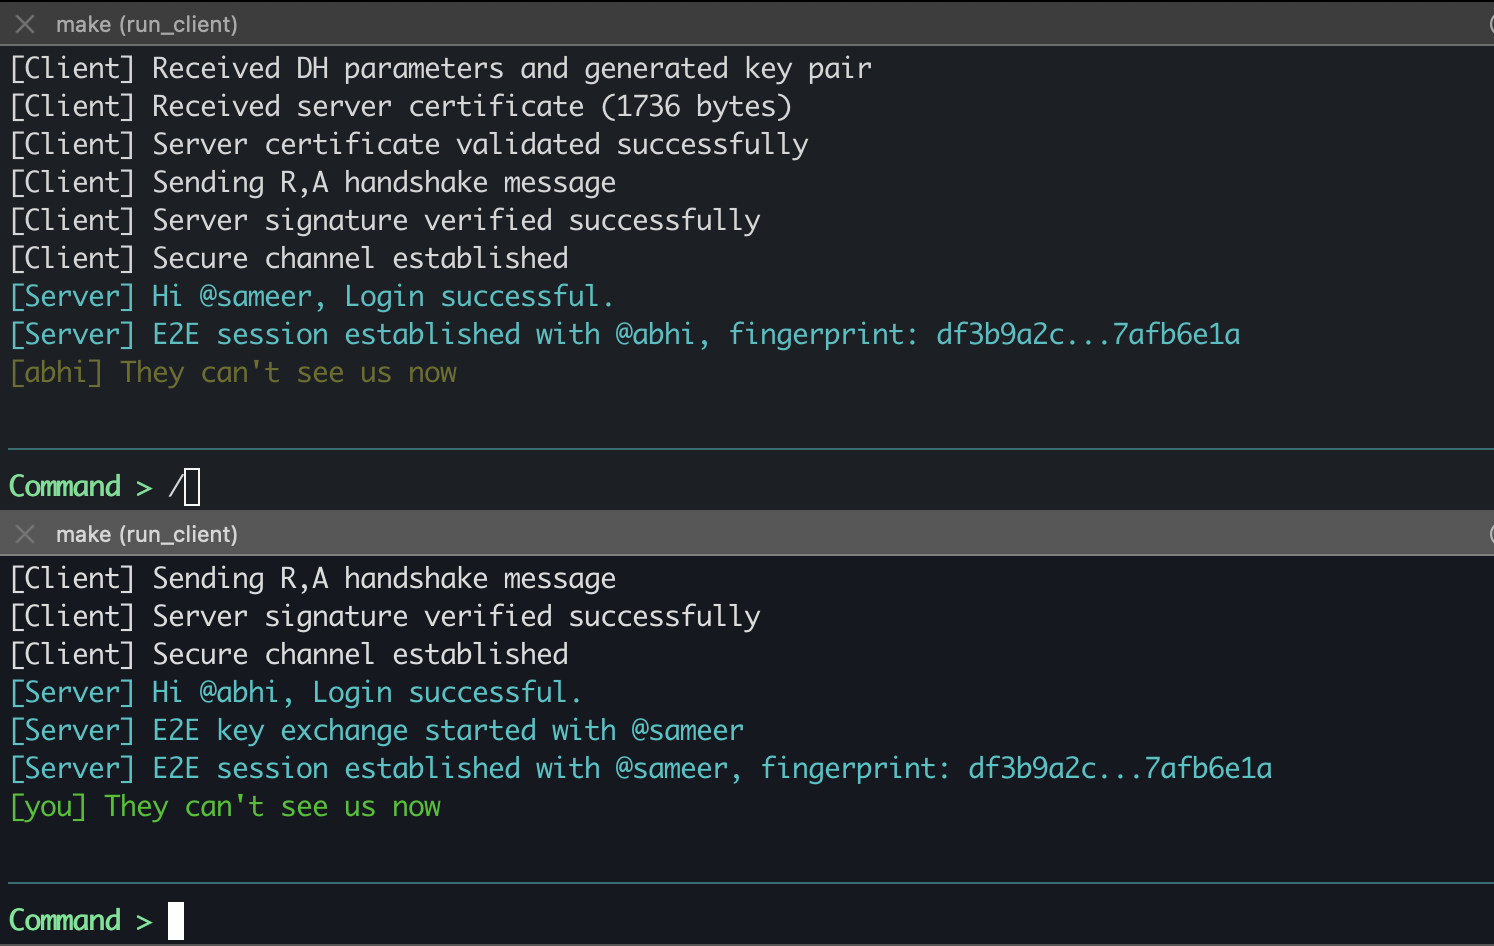
\includegraphics[width=0.6\linewidth]{images/phase4/fingerprint.png}
\caption{C1 and C2 derive the same end-to-end key.}
\end{figure}

\begin{figure}[H]
\centering
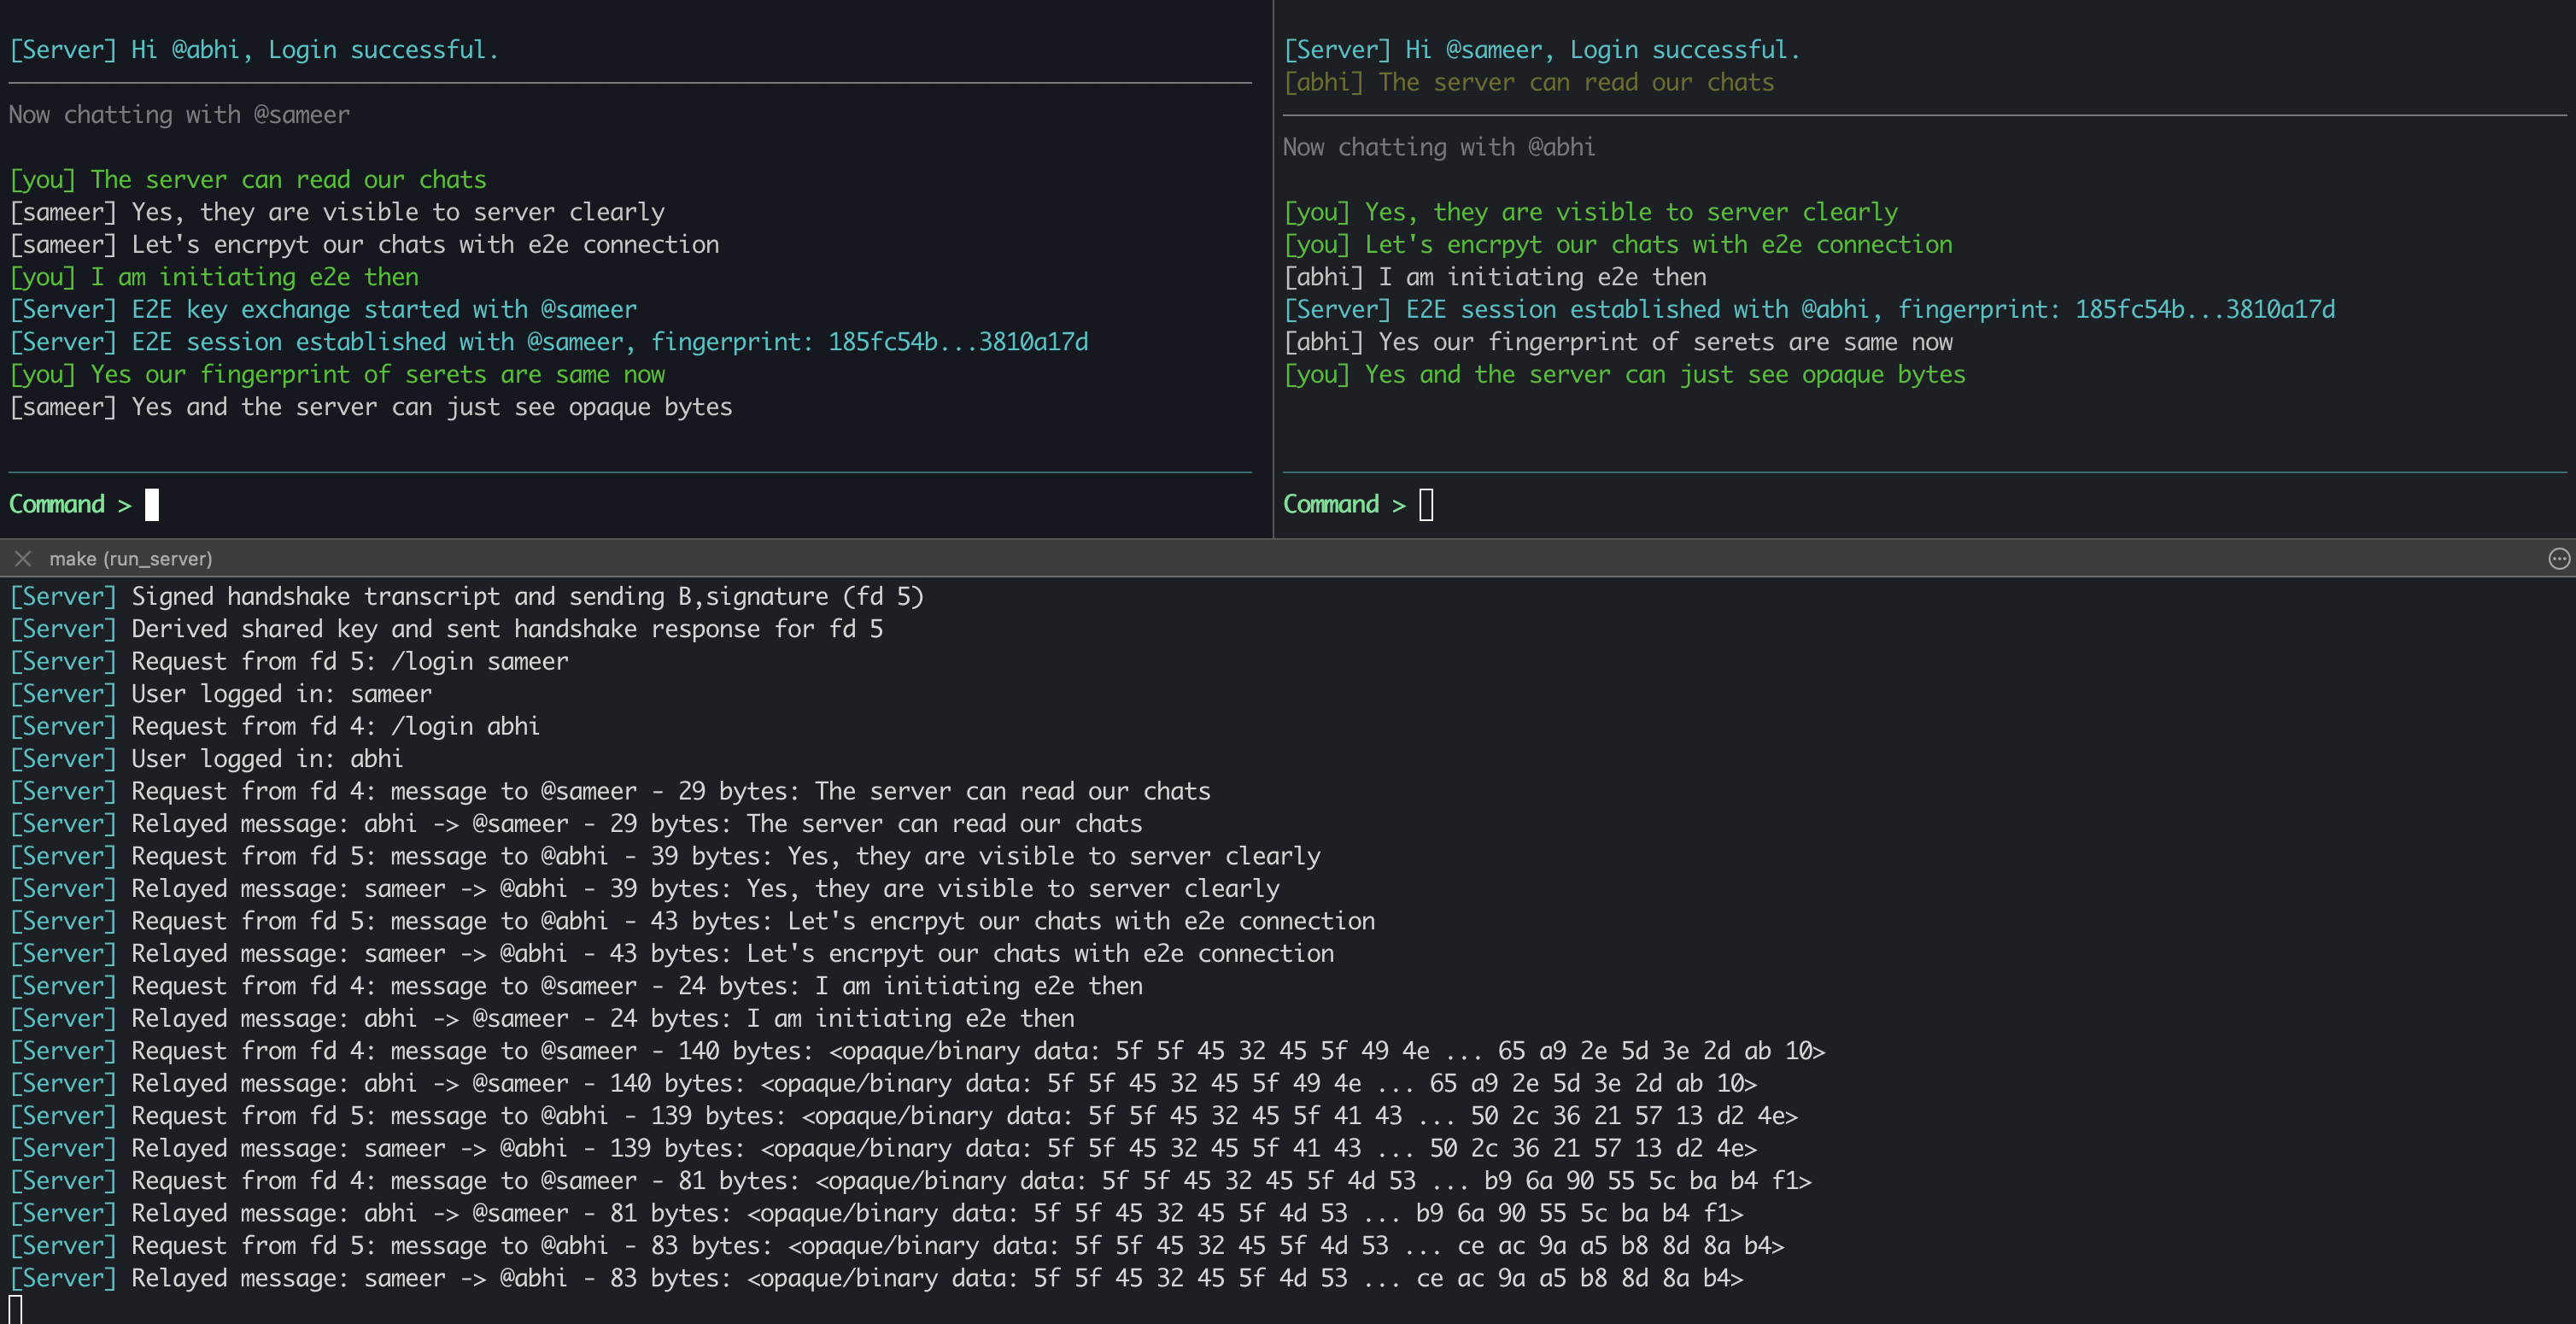
\includegraphics[width=\linewidth]{images/phase4/example.png}
\caption{\textbf{Demonstration of an End-to-End (E2E) Encrypted Chat Session.} The two clients (\texttt{abhi} and \texttt{sameer}) display the same fingerprint, confirming that they derived an identical shared secret without server involvement. The server log shows plaintext before E2E establishment but only opaque binary data afterwards, while both clients still decrypt and display the exchanged messages correctly.}
    \label{fig:e2e_verification}
\end{figure}

% =================================================
% PHASE 5
% =================================================
\section{Phase 5 -- Forward Secrecy}

\subsection{Rekey Design}

Phase~5 retains the Phase~4 E2E session but periodically replaces its session key. Each client maintains one \texttt{RekeyManager} for each peer. A rotation is due 60 seconds after session establishment and 60 seconds after every completed rotation.

The rotation proceeds as follows:

\begin{enumerate}
    \item The initiator generates a fresh DH keypair and sends its public value in an \texttt{\_\_E2E\_REKEY\_REQUEST\_\_}. This payload is encrypted with the \emph{current} AES key.
    \item The responder decrypts the request, generates its own fresh DH keypair, and derives a pending key
    \[
    K'=\mathrm{SHA256}(\mathrm{encode}(g^{a'b'}\bmod p)).
    \]
    It returns its public value and the SHA-256 fingerprint of $K'$ in an old-key-encrypted response message.
    \item The initiator derives its copy of $K'$, verifies the received fingerprint, and sends an old-key-encrypted \texttt{\_\_E2E\_REKEY\_CONFIRM\_\_} containing that fingerprint.
    \item The responder verifies the confirmation and installs $K'$. The initiator installs $K'$ after sending the confirmation, so both endpoints move to the same new key.
\end{enumerate}

The old AES key remains active during this short handshake, so ordinary chat messages continue to decrypt correctly. Once the switch completes, the old key and pending key material are overwritten and never reused.

\subsubsection{Avoiding Competing Rotations}

Only the lexicographically smaller username may initiate a timer-driven rotation for a given peer; in the code, \texttt{username >= peer} skips \texttt{begin\_rekey}. In addition, a request is rejected whenever \texttt{rekeyPending} is already set. These checks prevent two simultaneous DH exchanges and ensure that both clients converge on one fingerprint-verified pending key. After a successful rotation, each client logs the local timestamp and truncated fingerprint of the new key (\texttt{xxxxxxxx...yyyyyyyy}).

\subsection{Rotation Verification}

The following observations verify the rotation mechanism:

\begin{itemize}
    \item At E2E session establishment, both clients print the initial key fingerprint.
    \item Each completed rotation logs the peer, timestamp, and new key fingerprint.
    \item For at least two rotations, the fingerprint changes from the preceding generation.
    \item After each rotation, C1 and C2 display the same truncated fingerprint, demonstrating that they installed the same key.
\end{itemize}

\begin{figure}[H]
\centering
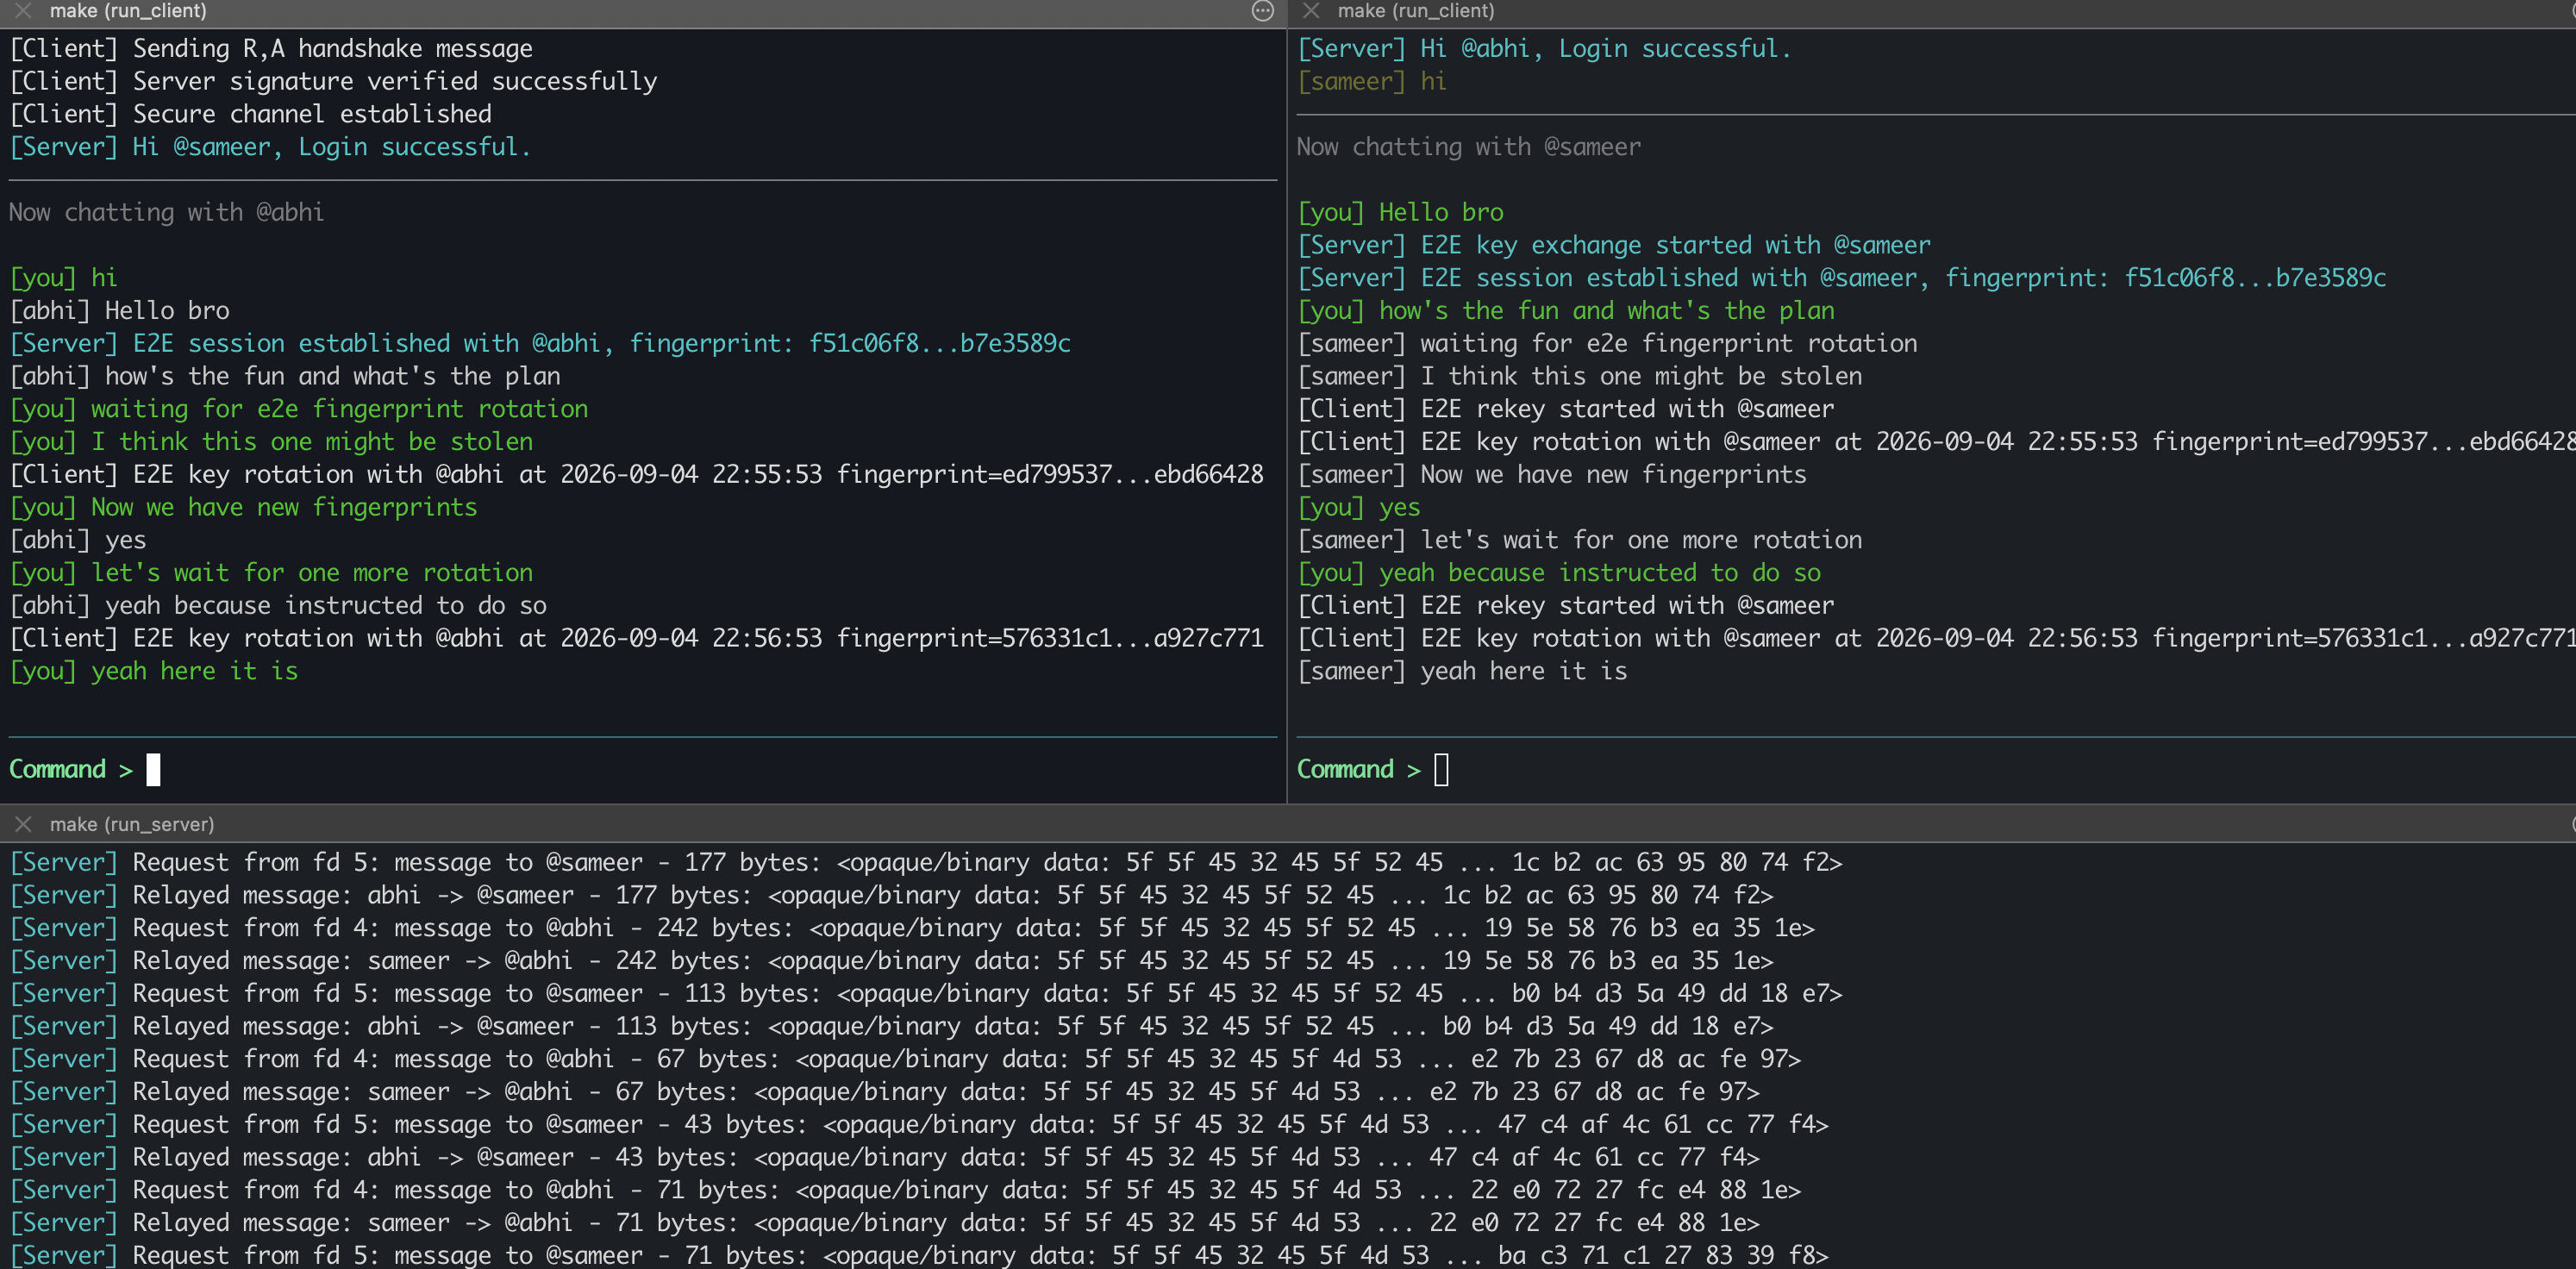
\includegraphics[width=\linewidth]{images/phase5/relay_e2e.png}

\caption{\textbf{Demonstration of Phase 5 Forward Secrecy and Automatic Key Rotation.} The clients (\texttt{sameer} and \texttt{abhi}) communicate through the relay server. Their logs show the initial E2E fingerprint and two 60-second rotations, with a different but matching fingerprint at each client after every rotation. Messages sent afterwards are correctly decrypted, while the server continues to route only opaque ciphertext.}
    \label{fig:forward_secrecy_rotation}
\end{figure}

\subsection{What Forward Secrecy Adds}

Phase~4 used one long-lived E2E AES key for the entire chat. Thus, an attacker who later obtained that key and had saved ciphertext from the server or network could decrypt all earlier traffic from that session.

Phase~5 limits the consequence of such a leak:

\begin{itemize}
    \item Each rotation creates an independent DH-derived key and discards the previous generation.
    \item Compromising one current session key exposes only messages encrypted in that key's lifetime, including stored ciphertext from that window.
    \item Earlier message generations remain protected because their DH secrets and AES keys have been discarded.
\end{itemize}

This is the forward-secrecy benefit: a later key compromise does not reveal earlier transcripts. It does not protect messages sent while the compromised key is active, nor does it help if an attacker can also obtain future keys while they are in use.

% =================================================
% APPENDIX
% =================================================
\appendix
\section{Generative AI Prompt Log}

The assignment requires all prompts used with generative AI to be documented. To maintain a compact format while providing full transparency, the complete conversation transcripts for major architectural and conceptual queries have been provided via shared links below.

\subsection*{ChatGPT \& Gemini Conversations}
\begin{itemize}
    \item \textbf{ChatGPT Session 1:} \url{https://chatgpt.com/share/6a9b0654-8c80-83ee-8e3f-2622d63aa401}
    \item \textbf{ChatGPT Session 2:} \url{https://chatgpt.com/share/6a9b066f-1a10-83ee-b55d-270e5c908648}
    \item \textbf{Gemini Session 1:} \url{https://share.gemini.google/B1MyfqSHY1Oj}
    \item \textbf{Gemini Session 2:} \url{https://share.gemini.google/adG0N6tk50ko}
    \item \textbf{Gemini Session 3:} \url{https://share.gemini.google/FFNaJH599q77}
\end{itemize}

\subsection*{GitHub Copilot Usage}
GitHub Copilot was actively used within the IDE throughout the development of all phases. Due to the ephemeral and fragmented nature of in-editor chat and autocomplete data, a raw prompt export is unavailable. Its usage primarily consisted of:
\begin{itemize}
    \item Routine coding, standard library syntax assistance, and auto-completion.
    \item Inline debugging and error resolution.
    \item Assistance in designing and formatting the terminal UI for the chat client.
\end{itemize}

\end{document}
